%%%%%%%%%%%%%%%%%%%% author.tex %%%%%%%%%%%%%%%%%%%%%%%%%%%%%%%%%%%
%
% sample root file for your "contribution" to a contributed volume
%
% Use this file as a template for your own input.
%
%%%%%%%%%%%%%%%% Springer %%%%%%%%%%%%%%%%%%%%%%%%%%%%%%%%%%


% RECOMMENDED %%%%%%%%%%%%%%%%%%%%%%%%%%%%%%%%%%%%%%%%%%%%%%%%%%%
\documentclass[graybox]{svmult}

% choose options for [] as required from the list
% in the Reference Guide

\usepackage{mathptmx}       % selects Times Roman as basic font
\usepackage{helvet}         % selects Helvetica as sans-serif font
\usepackage{courier}        % selects Courier as typewriter font
\usepackage{type1cm}        % activate if the above 3 fonts are
                            % not available on your system
%
\usepackage{makeidx}         % allows index generation
\usepackage{graphicx}        % standard LaTeX graphics tool
                             % when including figure files
\usepackage{multicol}        % used for the two-column index
\usepackage[bottom]{footmisc}% places footnotes at page bottom

\usepackage{amsmath,amssymb,color,url}

% see the list of further useful packages
% in the Reference Guide

\makeindex             % used for the subject index
                       % please use the style svind.ist with
                       % your makeindex program

%%%%%%%%%%%%%%%%%%%%%%%%%%%%%%%%%%%%%%%%%%%%%%%%%%%%%%%%%%%%%%%%%%%%%%%%%%%%%%%%%%%%%%%%%

\begin{document}

\title*{Complex network analysis of recurrences}
% Use \titlerunning{Short Title} for an abbreviated version of
% your contribution title if the original one is too long
\author{Reik V. Donner, Jonathan F. Donges, Yong Zou and Jan H. Feldhoff}
% Use \authorrunning{Short Title} for an abbreviated version of
% your contribution title if the original one is too long
\institute{Reik V. Donner \at Potsdam Institute for Climate Impact Research, Telegrafenberg A31, 14473 Potsdam, Germany, and Max Planck Institute for Biogeochemistry, Hans-Kn\"oll-Stra{\ss}e 10, 07745 Jena, Germany, \email{reik.donner@pik-potsdam.de}
\and Jonathan F. Donges \at Potsdam Institute for Climate Impact Research, Telegrafenberg A31, 14473 Potsdam, Germany, and Stockholm Resilience Centre, Stockholm University, Kr\"aftriket 2B, 11419 Stockholm, Sweden, \email{donges@pik-potsdam.de}
\and Yong Zou \at Department of Physics, East China Normal University, 200062 Shanghai, China,
and Potsdam Institute for Climate Impact Research, Telegrafenberg A31, 14473 Potsdam, Germany, \email{yzou@phy.ecnu.edu.cn}
\and Jan H. Feldhoff \at Potsdam Institute for Climate Impact Research, Telegrafenberg A31, 14473 Potsdam, Germany, and Department of Physics, Humboldt University, Newtinstra{\ss}e 15, 12489 Berlin, Germany, \email{feldhoff@pik-potsdam.de}
}
%
% Use the package "url.sty" to avoid
% problems with special characters
% used in your e-mail or web address
%
\maketitle

\abstract*{We present a complex network-based approach to characterizing the geometric properties of chaos by exploiting the pattern of recurrences in phase space. For this purpose, we utilize the basic definition of a recurrence as the mutual proximity of two state vectors in phase space (disregarding time information) and re-interpret the recurrence plot as a graphical representation of the adjacency matrix of a random geometric graph governed by the system's invariant density. The resulting recurrence networks contain exclusively geometric information about the system under study, which can be exploited for inferring quantitative information on the geometric properties of the system's attractor without explicitly studying scaling characteristics as in case of ``classical'' fractal dimension estimates.\\
Similar as the established recurrence quantification analysis, recurrence networks can be utilized for studying dynamical transitions in non-stationary systems, as well as for automatically discriminating between chaos and order without the necessity of extensive computations typically necessary when inferring this distinction based on the systems' maximum Lyapunov exponents. %For some well-studied model systems displaying complex transition cascades between chaos and ordered dynamics, we demonstrate that the novel complex network based characteristics display a somewhat better discriminative power than classical measures of RQA. However, this result should be taken with care, since both frameworks rely on established statistical properties, which are not necessarily best-suited for obtaining a clear distinction between both types of dynamics, as well as between different degrees of chaos.
Moreover, we provide a thorough re-interpretation of two bi- and multivariate generalizations of recurrence plots in terms of complex networks, which allow tracing geometric signatures of asymmetric coupling and complex synchronization processes between two or more chaotic oscillators.}

\abstract{We present a complex network-based approach to characterizing the geometric properties of chaos by exploiting the pattern of recurrences in phase space. For this purpose, we utilize the basic definition of a recurrence as the mutual proximity of two state vectors in phase space (disregarding time information) and re-interpret the recurrence plot as a graphical representation of the adjacency matrix of a random geometric graph governed by the system's invariant density. The resulting recurrence networks contain exclusively geometric information about the system under study, which can be exploited for inferring quantitative information on the geometric properties of the system's attractor without explicitly studying scaling characteristics as in case of ``classical'' fractal dimension estimates.\\
Similar as the established recurrence quantification analysis, recurrence networks can be utilized for studying dynamical transitions in non-stationary systems, as well as for automatically discriminating between chaos and order without the necessity of extensive computations typically necessary when inferring this distinction based on the systems' maximum Lyapunov exponents. %For some well-studied model systems displaying complex transition cascades between chaos and ordered dynamics, we demonstrate that the novel complex network based characteristics display a somewhat better discriminative power than classical measures of RQA. However, this result should be taken with care, since both frameworks rely on established statistical properties, which are not necessarily best-suited for obtaining a clear distinction between both types of dynamics, as well as between different degrees of chaos.
Moreover, we provide a thorough re-interpretation of two bi- and multivariate generalizations of recurrence plots in terms of complex networks, which allow tracing geometric signatures of asymmetric coupling and complex synchronization processes between two or more chaotic oscillators.}


\section{Introduction}

With the recent increase in available computational capacities and rising data volumes in various fields of science, complex networks have become an interesting and versatile tool for describing structural interdependencies between mutually interacting units \cite{Albert2002,Boccaletti2006,Costa2007,Newman2003}. Besides ``classical'' areas of research (such as sociology, transportation systems, computer sciences, or ecology), where these units are clearly (physically) identifiable, the success story of complex network theory has recently lead to a variety of ``non-conventional'' applications. 

One important class of such non-traditional applications of complex network theory are \emph{functional networks}, where the considered connectivity does not necessarily refer to ``physical'' vertices and edges, but reflects statistical interrelationships between the dynamics exhibited by different parts of the system under study. The term ``functional'' was originally coined in neuroscientific applications, where contemporaneous neuronal activity in different brain areas is often recorded using a set of standardized EEG channels. These data can be used for studying statistical interrelationships between different brain regions when performing certain tasks, having the idea in mind that the functional connectivity reflected by the strongest statistical dependencies can be taken as a proxy for the large-scale anatomic connectivity of different brain regions \cite{Zhou2006,Zhou2007}. Similar approaches have been later utilized for identifying dominant interaction patterns in other multivariate data sets, such as climate data \cite{Donges2009b,Donges2009a,Tsonis2004}.

Besides functional networks derived from multivariate time series, there have been numerous efforts for utilizing complex network approaches for quantifying structural properties of individual time series. In the last decade, several conceptually different approaches have been developed, see \cite{Donner2011IJBC} for a recent review. One important class of approaches make use of ideas from symbolic dynamics and stochastic processes by discretizing the dynamics and then studying the transition probabilities between the obtained groups in some Markov chain-like approach \cite{Nicolis2005}. A second class are visibility graphs and related concepts, which characterize some local convexity or record-breaking property within univariate time series data \cite{Donner2012AG,Lacasa2008,Luque2009}. The latter approach has important applications, such as providing new estimates of the Hurst exponent of fractal and multi-fractal stochastic processes \cite{Lacasa2009,Ni2009} or statistical tests for time series irreversibility \cite{Donges2013EPL,Lacasa2012}. Finally, a third important class of time series networks make use of similarities or proximity relationships between different parts of a dynamical system's trajectory \cite{Donner2011IJBC}, including such diverse approaches as cycle networks \cite{Zhang2006}, correlation networks \cite{Yang2008}, and phase space networks based on a certain definition of nearest neighbors \cite{Xu2008}. One especially important example of proximity networks are recurrence networks (RNs) \cite{Donner2010PRE,Donner2010NJP,Marwan2009}, which provide a reinterpretation of recurrence plots in network-theoretic terms and are already widely applied in a variety of fields.

In this chapter, we review the current state of knowledge on the theoretical foundations and potential applications of recurrence networks. We demonstrate that this type of time series networks naturally arise as random geometric graphs in the phase space of dynamical systems, which determines their structural characteristics and gives rise to a dimensionality interpretation of clustering coefficients and related concepts. In this spirit, the rich toolbox of complex network measures \cite{Boccaletti2006,Costa2007,Newman2003} provides various quantities that can be used for characterizing the system's dynamical complexity from some exclusively geometric viewpoint and allow discriminating between different types of dynamics. Beyond the single-system case, we also provide a corresponding in-depth discussion of cross- and joint recurrence plots from the complex network viewpoint. As a new aspect not previously reported in the literature, we provide a first-time theoretical treatment of a unification of single-system and cross-recurrence plots in a complex network context. Moreover, we discuss some new ideas related to the utilization of multivariate recurrence network-based approaches for studying geometric signatures of coupling and synchronization processes.


\section{From recurrence plots to recurrence networks}\label{sec:methods}

In this section, we introduce and discuss RNs as an alternative framework for studying recurrences in phase space from a geometric point of view. We start with the basic setting suitable for single dynamical systems, followed by some detailed considerations on two different multivariate generalizations, taking advantage of corresponding recent extensions \cite{Zbilut1998,Romano2004PLA} of the recurrence plot (RP) concept \cite{Eckmann1987,marwan2007}. Moreover, we provide a short overview on complex network characteristics and their meaning for RNs, highlighting the type of information that can be obtained using this approach -- as opposed to other recurrence based techniques like recurrence quantification analysis (RQA) \cite{zbilut92,trulla96}, recurrence time statistics, or estimation of dynamical invariants from RPs.

In the remainder of this chapter, the properties of all approaches to be discussed will be illustrated for the specific example of a R\"ossler system \cite{Roessler1976}
\begin{equation}
\left( \begin{array}{c}\dot{x}\\ \dot{y}\\ \dot{z}\end{array} \right) = \left( \begin{array}{c} -y-z\\ x+ay\\ b+z(x-c) \end{array} \right),
\label{eq:roessler}
\end{equation}
\noindent
where $a$, $b$ and $c$ are control parameters of the system, which will be varied if necessary. In the ``canonical'' case, $a=0.15$, $b=0.2$ and $c=10$. An example trajectory on the system's chaotic attractor at these parameter values is shown in Fig.~\ref{fig:attractor}. A similar phase-coherent attractor\footnote{Here, phase-coherent means chaotic oscillations around a well-defined center in a suitably chosen two-dimensional projection of the system~\cite{Zou2012aChaos,Zou2012bChaos}, whereas such projection is not possible in the funnel regime.} can be observed at $a=0.16$, $b=0.1$ and $c=8.5$, whereas for $a=0.2925$, $b=0.1$ and $c=8.5$, the system exhibits a structurally different chaotic attractor, the so-called funnel regime. 

\begin{figure}
\centering
\resizebox{\textwidth}{!}{\includegraphics*{roessler_attractor.png}}
\caption{Example trajectory on the chaotic attractor of the R\"ossler system (Eq.~\ref{eq:roessler}) at the canonical parameter values.}
\label{fig:attractor}
\end{figure}

For the multivariate extensions, we consider the paradigmatic case of two slightly detuned R\"ossler systems (i.e., otherwise identical systems whose natural oscillation frequencies differ from each other) that are diffusively coupled via their second ($y$) component:
\begin{equation}
\begin{split}
\dot{x}^{(1)} &= -(1+\nu)y^{(1)} - z^{(1)} \\
\dot{y}^{(1)} &= (1+\nu)x^{(1)} + ay^{(1)} + \mu_{21}(y^{(2)}-y^{(1)}) \\
\dot{z}^{(1)} &= b+z^{(1)}(x^{(1)}-c) \\
\dot{x}^{(2)} &= -(1-\nu)y^{(2)} - z^{(2)} \\
\dot{y}^{(2)} &= (1-\nu)x^{(2)} + ay^{(2)} + \mu_{12}(y^{(1)}-y^{(2)}) \\
\dot{z}^{(2)} &= b+z^{(2)}(x^{(2)}-c).
\end{split}
\label{eq:coupled_roessler}
\end{equation}
\noindent
Here, $\nu$ measures the detuning, $\mu_{kl}$ is the coupling strength with which system $k$ acts on system $l$ ($k,l\in\{1,2\}$), and the control parameters $a$, $b$, $c$ are chosen as being identical for both systems. A natural extension is taking different parameter values for both coupled systems, e.g., studying the situation with one phase-coherent and one funnel system coupled to each other.

In what follows, trajectories are generated using numerical integration of Eq.~(\ref{eq:roessler}) with a step size of $h=0.001$. As far as univariate (single-system) analyses are concerned, we will utilize the canonical parameter values, whereas we will study the attractors of the phase-coherent and funnel regime at the above given parameters in the coupled systems setting.
 


\subsection{Recurrence networks from single dynamical systems}\label{sec:rn}

\subsubsection{Basic idea}\label{sec:rn_idea}

As in the classical RP analysis, we start with a (possibly multivariate) time series $\{x_i\}_{i=1}^N$ with $x_i=x(t_i)$, which we interpret as a finite representation of the trajectory of some (deterministic or stochastic) dynamical system. For a discrete system (map), the sampling of the time series is directly given by the map, whereas for a continuous-time system, the time series values correspond to a temporally discretized sampling of a finite part of one trajectory of the system determined by some initial conditions. In the case of observation functions not representing the full variety of dynamically relevant components, we additionally assume that attractor reconstruction has been performed (e.g., using time-delay embedding or some related technique) \cite{Fraser1986,kantz1997,Kennel1992,Takens1981} and that the $x_i$ are state vectors in the corresponding (reconstructed) phase space of the dynamical system under study. 

From the set of (original or reconstructed) state vectors representing a discrete sampling of the underlying system's trajectory (e.g., the chaotic attractor of a dissipative system), we compute the recurrence matrix $\textbf{R}$ in the standard way \cite{Eckmann1987,marwan2007} as
\begin{equation}
R_{ij}(\varepsilon)=\Theta(\varepsilon-\|x_i-x_j\|),
\end{equation}
\noindent
where $\|\cdot\|$ can be any norm in phase space (e.g., Manhattan, Euclidean, or maximum norm). For convenience, we will use the maximum norm in all following examples.

We can re-interpret the mathematical structure $\textbf{R}(\varepsilon)$ as the adjacency matrix of some adjoint complex network embedded in phase space by setting
\begin{equation}
\mathbf{A}(\varepsilon)=\mathbf{R}(\varepsilon)-\mathbf{1}_N,
\label{eq:rn_definition}
\end{equation}
\noindent
where $\mathbf{1}_N$ is the $N$-dimensional identity matrix. The complex network defined this way is called \emph{$\varepsilon$-recurrence network (RN)}, as opposed to other types of proximity-based networks in phase space making use of different definitions of geometric closeness, e.g., considering $k$-nearest neighbors~\cite{Donner2011IJBC}. Specifically, the sampled state vectors $\{x_i\}$ are interpreted as vertices of a complex network, which are connected by undirected edges if they are mutually close in phase space (i.e., describe recurrences). Notably, the binary matrix $\mathbf{A}(\varepsilon)$ retains the symmetry properties of $\mathbf{R}(\varepsilon)$, which implies that the RN is a \emph{simple graph}, i.e., a complex network without multiple edges or self-loops (note that $A_{ii}=0$ according to definition~(\ref{eq:rn_definition})). For an example of a RP and associated RN, see Fig.~\ref{fig:example_rp_rn}. 

\begin{figure}
\centering
\resizebox{\textwidth}{!}{\includegraphics*{roessler_rp_and_rn.pdf}}
\caption{(A) Recurrence plot and (B) recurrence network for some finite trajectory ($N=200$, downsampled to a sampling interval of $\Delta t=1.0$) of the R\"ossler system (Eq.~\ref{eq:roessler}). Recurrences have been defined using maximum norm with a recurrence threshold $\varepsilon$ resulting in a recurrence rate of $RR=0.05$. The visual network representation has been obtained using a force-directed placement algorithm using the free software GEPHI. Vertex colors indicate the respective vertex degree in the network (orange: high degree, blue: low degree). Note that due to the peculiar three-dimensional structure of the R\"ossler attractor, the original attractor shape is not very well recovered by the network obtained from the short realization (this is distinctively different for other chaotic systems with a more two-dimensional structure, e.g., the Lorenz system~\cite{Donner2011IJBC}). %In the example, the formation of five densely connected clusters is probably due to the choise of the sampling time being close to co-prime with the mean oscillation frequency of the system, leading to groups of mutually close state vectors.
}
\label{fig:example_rp_rn}
\end{figure}


\subsubsection{Complex network characteristics}\label{sec:rn_measures}

Based on the re-interpretation of the recurrence matrix $\mathbf{R}(\varepsilon)$ as the adjacency matrix of an adjoint RN, we can utilize the large toolbox of complex network measures~\cite{Albert2002,Boccaletti2006,Costa2007,Newman2003} for characterizing the structural organization of a dynamical system in its phase space. Notably, this viewpoint is complementary to other concepts of nonlinear time series analysis making use of RPs. For example, RQA characterizes the statistical properties of line structures in the RP, which implies explicit consideration of dynamical aspects (i.e., sequences of state vectors). In turn, RNs do not make use of time information, since network properties are generally invariant under vertex relabelling (i.e., permutations of the order of observations)~\cite{Donner2010NJP}. In this spirit, RN analysis provides geometric instead of dynamical characteristics. This idea of a geometric analysis is similar to some classical concepts of fractal dimensions (e.g., box-counting or correlation dimensions), where certain scaling laws in dependence on the spatial scale of resolution (corresponding here to $\varepsilon$) are exploited. In turn, RN analysis can be performed (as RQA) using only a single fixed scale ($\varepsilon$) instead of explicitly studying scaling properties over a range of threshold values.

The distinction between dynamical and geometric information implies that in case of RN analysis, the typical requirement of a reasonable (typically uniform) temporal sampling of the considered trajectory is replaced by the demand for a suitable spatial coverage of the system's attractor in phase space. Specifically, under certain conditions the latter could also be obtained by considering an ensemble of short trajectories instead of a single long one. If the trajectory under study is relatively densely sampled, trivial serial correlations can lead to a selection bias in the set of sampled state vectors; the latter could be avoided by reasonable downsampling. In the same context, the possibility of utilizing Theiler windows for removing edges representing short-term auto-correlations (e.g., recurrence points close to the main diagonal in the RP) should be mentioned as another strategy based on a somewhat different rationale~\cite{Donner2010NJP}. However, from a conceptual perspective, downsampling can provide an unbiased sampling of the attractor as long as the fixed sampling time does not correspond to any integer multiple of some of the system's natural frequencies. As an alternative, bootstrapping from the set of available state vectors provides another feasible option, which should be prefered if a sufficiently long time series is available. In general, numerical experiments and different applications suggest that stable estimates of RN characteristics can often already be obtained using a sample size of $N\sim\mathcal{O}(10^2\dots 10^3)$ data points~\cite{Donges2011NPG,Donges2011PNAS}.

When considering quantitative characteristics of complex networks, different classifications of measures are possible. First, we may distinguish measures based on the concept of graph neighborhoods from those making use of shortest path-based characteristics. (This is not an exhaustive classification, since it potentially neglects other important network measures, e.g., such based on diffusion processes or random walks on the network.) Second, network measures can be classified into such making use of local, meso-scale and global information. This scheme is widely equivalent to the first one in that local information refers to properties determined by the graph neighborhood of a given vertex, whereas global information takes contributions due to all vertices of the network into account, which is common for shortest path-based measures. Finally, we can differentiate between measures quantifying properties of single vertices, pairs of vertices, and the network as a whole. In this chapter, we will utilize the latter way of classification, since it appears most instructive from the applied point of view (i.e., we are commonly interested in either the local or the global geometry of an attractor).

In what follows, we will denote all properties computed from a RN consisting of a finite number $N$ of state vectors as $\hat{f}$, pointing to the fact that they are estimated from a given sample of state vectors but shall characterize the entire trajectory of the system under study. We will discuss a corresponding continuous framework generalizing all network characteristics described below in Section~\ref{sec:analytics}. In order to focus the following discussion, we review only the possibly most relevant characteristics associated with RNs. More details including further measures can be found in \cite{Donges2012PRE,Donner2010NJP}.


\subsubsection{Shortest paths in recurrence networks}

In addition to the concepts of vertices (in the RN, the state vectors of a sampled dynamical system) and edges (recurrences between state vectors in phase space), the notion of shortest paths is a third important ingredient in complex network theory. 

In general, a \emph{path} between two specified vertices $i$ and $j$ is an ordered sequence of edges starting at $i$ and ending at $j$, with its \emph{path length} $\hat{l}_{ij}(\varepsilon)$ given by the number of edges in this sequence. In the context of RNs, we can thus understand a path as a sequence of mutually overlapping $\varepsilon$-balls\footnote{Here, $\varepsilon$-balls refers to general (hyper-)volumes according to the specific norm chosen for measuring distances in phase space, e.g., hypercubes of edge length $2\varepsilon$ in case of the maximum norm, or hyperballs of radius $\varepsilon$ for the Euclidean norm.} $B_{\varepsilon}(x_i),B_{\varepsilon}(x_{k_1}),\dots,B_{\varepsilon}(x_{k_{l_{i,j}-1}}),B_{\varepsilon}(x_j)$, where $$B_{\varepsilon}(x)=\{y\,|\,\|x-y\|<\varepsilon\}$$ is an open set describing a volume with maximum distance $\varepsilon$ (measured in a given norm) from $x$, and $B_{\varepsilon}(x_i)\cap B_{\varepsilon}(x_{k_1})\neq\emptyset,\dots,B_{\varepsilon}(x_{k_{l_{i,j}-1}})\cap B_{\varepsilon}(x_j)\neq\emptyset$.

Following these considerations, a \emph{shortest path} is a minimum sequence of edges (mutually overlapping $\varepsilon$-balls) between two fixed vertices (state vectors) $i$ and $j$. Note that a shortest path does not need to be unique. In turn, due to the discrete character of a network, it is rather typical that there are multiple shortest paths between some specific pair of vertices. In what follows, the shortest path length will be denoted as $\hat{d}_{ij}$, and the multiplicity of such shortest paths as $\hat{\sigma}_{ij}$.


\subsubsection{Local (vertex-based) measures}

The conceptually simplest measure characterizing the connectivity properties of a single vertex in a complex network is the \textit{degree} or \textit{degree centrality}
\begin{equation}
\hat{k}_v(\varepsilon)=\sum_{i=1}^N A_{iv}(\varepsilon),
\label{eq:degree}
\end{equation}
\noindent
which simply counts the number of edges associated with a given vertex $v$. From the perspective of recurrences, it is reasonable to replace the degree by a normalized characteristic, the \textit{degree density}
\begin{equation}
\hat{\rho}_v(\varepsilon)=\frac{\hat{k}_v(\varepsilon)}{N-1}=\frac{1}{N-1} \sum_{i=1}^N A_{iv}(\varepsilon),
\label{eq:locrho}
\end{equation}
\noindent
which corresponds to the definition of the local recurrence rate of the state $x_v$. $\hat{\rho}_v(\varepsilon)$ quantifies the density of states in the $\varepsilon$-ball around $x_v$, i.e., the probability that a randomly chosen member of the available sample of state vectors is $\varepsilon$-close to $x_v$. An illustration of this fact for the R\"ossler system is presented in Fig.~\ref{fig:local}A; here, phase space regions with a high density of points (i.e., a high residence probability of the sampled trajectory) are characterized by a high degree density.

\begin{figure}
\centering
\resizebox{\textwidth}{!}{\includegraphics*{phase_deg_cc_cls_btw.pdf}}
\caption{Spatial distributions of vertex characteristics of the RN obtained for the R\"ossler system (Eq.~\ref{eq:roessler}) at the canonical parameters (RPs computed using the maximum norm with $\hat{\rho}=0.01$, $N=10,000$ and sampling time $\Delta t=0.2$): (A) degree centrality, (B) local clustering coefficient, (C) closeness centrality, (D) betweenness centrality.}
\label{fig:local}
\end{figure}

In order to characterize the density of connections among the neighbors of a given vertex $v$, we can utilize the \textit{local clustering coefficient}
\begin{equation}
\hat{\mathcal{C}}_v(\varepsilon)=\frac{1}{\hat{k}_v(\varepsilon)(\hat{k}_v(\varepsilon)-1)} \sum_{i,j=1}^N A_{vi}(\varepsilon) A_{ij}(\varepsilon) A_{jv}(\varepsilon),
\label{eq:locclustering}
\end{equation}
\noindent
which measures the fraction of pairs of vertices in the $\varepsilon$-ball around $x_v$ that are
mutually $\varepsilon$-close. For vertices with $\hat{k}_v(\varepsilon)<2$, we define $\hat{\mathcal{C}}_v(\varepsilon)=0$. It can be shown (see Section~\ref{sec:transitivity}) that the local clustering coefficient in a RN is associated with the geometric alignment of state vectors. Specifically, close to dynamically invariant objects such as unstable periodic orbits (UPOs) of low period, the dynamics of the system is effectively lower-dimensional, which results in a locally enhanced fraction of closed paths of length 3 (``triangles'') and, thus, a higher local clustering coefficicent. The latter behavior is exemplified in Fig.~\ref{fig:local}B for the R\"ossler system, where we recognize certain bands with higher values of $\hat{\mathcal{C}}_v$ corresponding to the positions of known low-periodic UPOs~\cite{Donner2010NJP}.

While degree and local clustering coefficient characterize network structures on the local and meso-scale, there are further vertex characteristics that make explicit use of the concept of shortest paths and, thus, provide measures relying on the connectivity of the entire network. Two specific properties of this kind are the \textit{closeness} or \textit{closeness centrality}
\begin{equation}
\hat{c}_v(\varepsilon)=\left(\frac{1}{N-1}\sum_{i=1}^N \hat{d}_{vi}(\varepsilon) \right)^{-1},
\label{eq:closeness}
\end{equation}
\noindent
which gives the inverse arithmetic mean of the shortest path lengths between vertex $v$ and all other vertices, and the \textit{local efficiency}
\begin{equation}
\hat{e}_v(\varepsilon)=\frac{1}{N-1}\sum_{i=1}^N \hat{d}_{vi}(\varepsilon)^{-1},
\label{eq:locefficiency}
\end{equation}
\noindent
which gives the inverse harmonic mean of these shortest path lengths. Notably, the latter quantity has the advantage of being well-behaved in the case of disconnected network components, where there are no paths between certain pairs of vertices (i.e., $\hat{d}_{ij}=\infty$). In order to circumvent divergences of the closeness due to the existence of disconnected components, it is convenient to always set $\hat{d}_{ij}$ to the highest possible value of $N-1$ for pairs of vertices that cannot be mutually reached. Both $\hat{c}_v(\varepsilon)$ and $\hat{e}_v(\varepsilon)$ characterize the geometric centrality of vertex $v$ in the network, i.e., closeness and local efficiency exhibit the highest values for such vertices which are situated in the center of the RN (see Fig.~\ref{fig:local}C for an illustration for the R\"ossler system).

Another frequently studied path-based vertex characteristic is the so-called \textit{betweenness} or \textit{betweenness centrality}, which measures the fraction of shortest paths in a network traversing a given vertex $v$. Let $\hat{\sigma}_{ij}$ denote the total number of shortest paths between two vertices $i$ and $j$ and $\hat{\sigma}_{ij}(v)$ the multiplicity of these paths that include a given vertex $v$, betweenness centrality is defined as
\begin{equation}
\hat{b}_v(\varepsilon)=\sum_{i,j=1; i,j\neq v}^M \frac{\hat{\sigma}_{ij}(v)}{\hat{\sigma}_{ij}}.
\label{eq:betweenness}
\end{equation}
\noindent
Betweenness centrality is commonly used for characterizing the importance of vertices for information propagation in networks. In the RN context, it can be interpreted as indicating the local degree of fragmentation of the underlying attractor~\cite{Donner2010NJP}. To see this, consider two densely populated regions of phase space that are separated by a poorly populated one. Vertices in the latter will ``bundle'' the shortest paths between vertices in the former ones, thus forming geometric bottlenecks in the RN. In this spirit, we may understand the spatial distribution of betweenness centrality for the R\"ossler system (Fig.~\ref{fig:local}D) which includes certain bands with higher and lower residence probability reflected in lower and higher betweenness values.


\subsubsection{Pairwise vertex and edge measures}

In contrast to vertices, whose properties can be characterized by a multitude of graph characteristics, there are fewer measures that explicitly relate to the properties of edges or, more general, pairs of vertices. One such measure is the \textit{matching index}, which quantifies the overlap of the network neighborhoods of two vertices $v$ and $w$:
\begin{equation}
\hat{m}_{vw}(\varepsilon)=\frac{\sum_{i=1}^N A_{vi}(\varepsilon) A_{wi}(\varepsilon)}{\hat{k}_v(\varepsilon)+\hat{k}_w(\varepsilon)-\sum_{i=1}^N A_{vi}(\varepsilon) A_{wi}(\varepsilon)}.
\label{eq:matching}
\end{equation}
\noindent
From the above definition, it follows that $\hat{m}_{vw}(\varepsilon)=0$ if $\|x_v-x_w\|\geq 2\varepsilon$. In turn, there can be mutually unconnected vertices $v$ and $w$ ($A_{vw}=0$) with $\varepsilon\leq \|x_v-x_w\|< 2\varepsilon$ that have some common neighbors and, thus, non-zero matching index. In the context of recurrences in phase space, $\hat{m}_{vw}(\varepsilon)=1$ implies that the states $x_v$ and $x_w$ are twins, i.e., share the same neighborhood in phase space. In this spirit, we interpret $\hat{m}_{vw}(\varepsilon)$ as the degree of twinness of two state vectors. Note that twins have important applications in creating surrogates for testing for the presence of complex synchronization~\cite{Thiel2006,Romano2009}.

While the concept of matching index does not require the presence of an edge between two vertices $v$ and $w$, there are other characteristics that are explicitly edge-based. To this end, we only mention that the concept of betweenness centrality can also be transfered to edges, leading to the \textit{edge betweenness} measuring the fraction of shortest paths on the graph traversing through a specific edge $(v,w)$:
\begin{equation}
\hat{b}_{vw}(\varepsilon)=\sum_{i,j=1; i,j\neq v,w}^M \frac{\hat{\sigma}_{ij}(v,w)}{\hat{\sigma}_{ij}},
\label{eq:edgebetweenness}
\end{equation}
\noindent
where $\hat{\sigma}_{ij}(v,w)$ gives the total number of shortest paths between two vertices $i$ and $j$ that include the edge $(v,w)$. If there is no edge between two vertices $v$ and $w$, we set $\hat{b}_{vw}=0$ for convenience. As the (vertex-based) betweenness centrality, in a RN edge betweenness characterizes the local fragmentation of the studied dynamical system in its phase space.

\begin{figure}
\centering
\resizebox{\textwidth}{!}{\includegraphics*{edge_based_measures.pdf}} 
\caption{Color-coded representations of (A) matching index $\hat{m}_{ij}$ and (B) logarithmic edge betweenness $\log_{10} \hat{b}_{ij}$ for the RN of the R\"ossler system (using $N=100$ vertices corresponding to a sampling with $\Delta t=1.0$, RP obtained using the maximum norm with $\varepsilon$ chosen such as to yield a recurrence rate of $RR=0.05$).}
\label{fig:edgemeasures}
\end{figure}

Figure~\ref{fig:edgemeasures} illustrates the two aforementioned concepts for one example trajectory of the R\"ossler system. As can be seen, there is no simple correspondence between matching index and edge betweenness, since both quantify distinctively different aspects of phase space geometry. Specifically, there are more pairs of vertices with non-zero matching index than edges, even though there are also pairs of vertices with $\hat{b}_{vw}(\varepsilon)>0$ but $\hat{m}_{vw}(\varepsilon)=0$ (i.e., there is an edge between $v$ and $w$, but both have no common neighbors). However, for those pairs of vertices for which both characteristics are non-zero, we find a clear anti-correlation. One interpretation of this finding is that a large matching index typically corresponds to very close vertices in phase space; such pairs of vertices can in turn be easily exchanged as members of shortest paths on the network, which implies lower edge betweenness values. A similar argument may explain the coincidence of high edge betweenness and low non-zero matching index values.


\subsubsection{Global network measures}

Some, but not all useful global network characteristics can be derived by averaging certain local-scale (vertex) properties. Prominently, the \textit{edge density}
\begin{equation}
\hat{\rho}(\varepsilon)=\frac{1}{N}\sum_{v=1}^N \hat{\rho}_v(\varepsilon)=\frac{1}{N(N-1)} \sum_{i,j=1}^N A_{ij}(\varepsilon)
\label{eq:edgedensity}
\end{equation}
\noindent
is defined as the arithmetic mean of the degree densities of all verticies and characterizes the fraction of possible edges that are present in the network. Notably, for a RN the edge density equals the recurrence rate $RR(\varepsilon)$ of the underlying RP\footnote{Strictly speaking, this is only true if the recurrence rate is defined such as the main diagonal in the RP is excluded in the same way as potential self-loops from the RN's adjacency matrix.}. It is trivial to show that $\hat{\rho}(\varepsilon)$ is a monotonically increasing function of the recurrence threshold $\varepsilon$: the larger the threshold, the more neighbors can be found, and the higher the edge density.

In a similar way, we can consider the arithmetic mean of the local clustering coefficients $\hat{\mathcal{C}}_v(\varepsilon)$ of all vertices, resulting in the (Watts-Strogatz) \textit{global clustering coefficient}~\cite{Watts1998}
\begin{equation}
\hat{\mathcal{C}}(\varepsilon)=\frac{1}{N}\sum_{v=1}^N \hat{\mathcal{C}}_v(\varepsilon)
= \frac{1}{N}\sum_{v=1}^N \frac{\sum_{i,j=1}^N A_{vi}(\varepsilon) A_{ij}(\varepsilon) A_{jv}(\varepsilon)}{\hat{k}_v(\varepsilon)(\hat{k}_v(\varepsilon)-1)}.
\label{eq:globclustering}
\end{equation}
\noindent
The global clustering coefficient measures the mean fraction of triangles that include the different vertices of the network. Given our interpretation of the local clustering coefficient in a RN, $\hat{\mathcal{C}}(\varepsilon)$ can be interpreted as a proxy for the average local dimensionality of the dynamical system in phase space.

Notably, in the case of a very heterogeneous degree distribution, the global clustering coefficient will be dominated by contributions from the most abundant type of vertices. For example, for a scale-free network with $p(k)\sim k^{-\gamma}$, vertices with small degree will contribute predominantly, which can lead to an underestimation of the actual fraction of triangles in the network, since $\hat{\mathcal{C}}_v(\varepsilon)=0$ if $\hat{k}_v(\varepsilon)<2$ by definition. In order to correct for such effects, Barrat and Weigt~\cite{Barrat2000} proposed an alternative definition of the clustering coefficient, which is nowadays frequently refered to as \textit{network transitivity}~\cite{Boccaletti2006} and is defined as
\begin{equation}
\hat{\mathcal{T}}(\varepsilon)= \frac{\sum_{v,i,j=1}^N A_{vi}(\varepsilon) A_{ij}(\varepsilon) A_{jv}(\varepsilon)}{\sum_{v,i,j=1}^N A_{vi}(\varepsilon) A_{jv}(\varepsilon)}.
\label{eq:transitivity}
\end{equation}
\noindent
When interpreting $\hat{\mathcal{C}}(\varepsilon)$ as a proxy for the average local dimensionality, $\hat{\mathcal{T}}(\varepsilon)$ characterizes the effective global dimensionality of the system.

Finally, turning to shortest path-based characteristics, we define the \textit{average path length}
\begin{equation}
\hat{\mathcal{L}}(\varepsilon)=\frac{1}{N(N-1)} \sum_{i,j=1}^N \hat{d}_{ij}(\varepsilon) = \frac{1}{N} \sum_{v=1}^N \hat{c}_v(\varepsilon)^{-1}
\label{eq:apl}
\end{equation}
\noindent
as the arithmetic mean of the shortest path lengths between all pairs of vertices, and the \textit{global efficiency}
\begin{equation}
\hat{\mathcal{E}}(\varepsilon)=\left(\frac{1}{N(N-1)} \sum_{i,j=1}^N \hat{d}_{ij}(\varepsilon)^{-1} \right)^{-1} = \left( \frac{1}{N} \sum_{v=1}^N \hat{e}_v(\varepsilon) \right)^{-1}
\label{eq:globefficiency}
\end{equation}
\noindent
as the associated harmonic mean. Notably, the average path length can be rewritten as the arithmetic mean of the inverse closeness, and the global efficiency as the inverse arithmetic mean of the local efficiency. We can easily convince ourselves that the average path length must exhibit an inverse relationship with the recurrence threshold, since it approximates (constant) distances in phase space in units of $\varepsilon$~\cite{Donner2010NJP}.


\subsection{Inter-system recurrence networks}\label{sec:irn}

In the last decade, two different widely applicable bi- and multivariate extensions of RPs and RQA have been proposed~\cite{marwan2007}: cross-recurrence plots~\cite{Marwan2002PLA,Zbilut1998} and joint recurrence plots~\cite{Romano2004PLA}. In the following, we discuss some possibilities for utilizing these approaches in a complex network framework, following previous considerations in~\cite{Feldhoff2011,Feldhoff2012,Feldhoff2013}. For this purpose, let us consider $K$ (possibly multivariate) time series $\{x_i^k\}_{i=1}^{N_k}$ with $x_i^k=x^k(t^k_i)$ sampled at times $\{t^k_i\}$ from dynamical systems $\{X_k\}$ with $k=1,\dots,K$. 

%{\color{red}need to mention MRP of Nichols et al. 2006 here as well?}


\subsubsection{Cross-recurrences and cross-recurrence networks}\label{sec:crn_idea}

One way of extending recurrence analysis to the study of multiple dynamical systems is looking at \emph{cross-recurrences}\footnote{It is important to realize that cross-recurrences are not to be understood in the classical sense of Poincar{\'e}'s considerations, since they do not indicate the return of an isolated dynamical system to some previously assumed state. In contrast, they imply an arbitrarily delayed close encounter of the trajectories of two \emph{distinct} systems and, therefore, should be better named \emph{cross encounters} instead. Following the same reasoning, terms such as \emph{cross-recurrence plot} or \emph{cross-recurrence rate} are suggestive, but potentially misleading. However, to comply with the existing literature on cross-recurrence plots, we will adopt the established terms even despite their conceptual ambiguities.}, \textit{i.e.}, encounters of the trajectories of two systems $X_k$ and $X_l$ sharing the same phase space, where $x_i^k \approx x_j^l$~\cite{Marwan2002PLA,Zbilut1998} (see Fig.~\ref{fig:sketch_cr_jr} for some illustration). Unlike the traditional recurrence matrix $\mathbf{R}$ of a single system, the elements of the cross-recurrence matrix $\mathbf{CR}^{kl}$ are defined as
\begin{equation}
CR_{ij}^{kl}(\varepsilon_{kl})=\Theta(\varepsilon_{kl} - \|x_i^k - x_j^l\|),
\end{equation}
where $i=1,\dots,N_k$, $j=1,\dots,N_l$, and $\varepsilon_{kl}$ is a prescribed threshold distance in the joint phase space of both systems. As in the single-system case, $\varepsilon_{kl}$ determines the number of mutual neighbors in phase space, quantified by the \emph{cross-recurrence rate}
\begin{equation}
RR_{kl}(\varepsilon_{kl})=\frac{1}{N_k N_l}\sum_{i=1}^{N_k} \sum_{j=1}^{N_l} CR_{ij}^{kl}(\varepsilon_{kl}),
\label{eq:crr}
\end{equation}
\noindent
which is a monotonically increasing function of $\varepsilon_{kl}$ (i.e., the larger the distance threshold in phase space, the more neighbors are found). Note that unlike $\mathbf{R}^k$ and $\mathbf{R}^l$, the cross-recurrence matrix $\mathbf{CR}^{kl}$ is asymmetric, since we typically have $\|x_i^k - x_j^l\|\neq\|x_i^l - x_j^k\|$. Even more, it can be non-square if time series of different lengths ($N_k\neq N_l$) are considered.

\begin{figure}
\centering
%\resizebox{0.9\textwidth}{!}{\includegraphics*{sketch_cr_jr.pdf}}
\resizebox{0.40\textwidth}{!}{\includegraphics*{crossrec01.pdf}} \hfill
\resizebox{0.54\textwidth}{!}{\includegraphics*{jointrec01.pdf}}
\caption{Schematic representation of the notions of cross-recurrence (left) and joint recurrence (right) between the trajectories $x(t)$ and $y(t)$ of two dynamical systems $X$ and $Y$. $PS_X$ and $PS_Y$ denote the individual phase spaces of systems $X$ and $Y$ within the joint recurrence framework, whereas $PS_{XY}$ indicates the joint phase space of $X$ and $Y$ necessary for considering cross-recurrences.}
\label{fig:sketch_cr_jr}
\end{figure}

Due to the aforementioned characteristics, $\mathbf{CR}^{kl}$ cannot be directly interpreted as the adjacency matrix of a network with similar properties as single-system RNs. This is because the indices $i$ and $j$ label two distinct sets of state vectors belonging to systems $X_k$ ($i$) and $X_l$ ($j$), respectively. In turn, we can interpret the state vectors $\{x^k_i\}$ and $\{x^l_j\}$ as two distinct groups of vertices, and $\mathbf{CR}^{kl}$ as being an adjacency matrix of a \emph{cross-recurrence network (CRN)} providing a binary encoding of the presence of edges between vertices belonging to different groups. This is the defining property of bipartite graphs~\cite{Newman2003}.

Bipartite networks are found in a wide range of fields~\cite{Guimera2007,Kitsak2011} and can be understood as a generic way for describing arbitrary complex networks~\cite{Guillaume2004,Guillaume2006}. The large variety of applications of bipartite graphs has triggered great interest in models describing their properties in an appropriate way. Particular attention has been spent on the problem of community detection~\cite{Fortunato2010}, involving new definitions for the modularity function~\cite{Barber2007,Guimera2007,Murata2009,Suzuki2009} and the development of proper algorithms for community detection~\cite{Barber2007,Du2008,Lehmann2008,Sawardecker2009}, partially relating to the spectral properties of the networks. However, their specific structure renders some traditional definitions of network-theoretic measures non-applicable, calling for generalizations or even re-definitions of quantities such as the clustering coefficient~\cite{Lind2005,Zhang2008PhysA}. This is why we do not further consider explicit quantification of the properties of the bipartite CRN, but follow a different approach detailed below.


\subsubsection{Combining single-system and cross-recurrence networks}\label{sec:irn_idea}

As mentioned in Section~\ref{sec:crn_idea}, there is a lack of appropriate measures for characterizing explicit bipartite network structures as compared with the rich toolbox of general-purpose complex network characteristics~\cite{Boccaletti2006,Costa2007}. Therefore, instead of explicitly investigating the bipartite structure of the CRN, it is more useful to combine the information contained in the single-system recurrence matrices $\mathbf{R}^k(\varepsilon_k)$ and the cross-recurrence matrices $\mathbf{CR}^{kl}(\varepsilon_{kl})$ to construct an inter-system recurrence matrix~\cite{Feldhoff2012}
\begin{equation}
\mathbf{IR}(\mathbf{\varepsilon})=\left( \begin{array}{cccc} \mathbf{R}^1(\varepsilon_{11}) & \mathbf{CR}^{12}(\varepsilon_{12}) & \hdots & \mathbf{CR}^{1K}(\varepsilon_{1K}) \\
\mathbf{CR}^{21}(\varepsilon_{21}) & \mathbf{R}^2(\varepsilon_{22}) & \hdots & \mathbf{CR}^{2K}(\varepsilon_{2K}) \\
\vdots & \vdots & \ddots & \vdots \\ \mathbf{CR}^{K1}(\varepsilon_{K1}) & \mathbf{CR}^{K2}(\varepsilon_{K2}) & \hdots & \mathbf{R}^K(\varepsilon_{KK}) \end{array} \right).
\label{isrm}
\end{equation}
Here, $\mathbf{\varepsilon}=(\varepsilon_{kl})_{kl}$ is a $K \times K$ matrix containing the single-system recurrence thresholds $\varepsilon_{kk}=\varepsilon_k$ and (cross-recurrence) distance thresholds $\varepsilon_{kl}$. The corresponding \emph{inter-system recurrence network (IRN)}~\cite{Feldhoff2012} (see Fig.~\ref{fig:irn_example} for an example) is fully described by its adjacency matrix
\begin{equation}
\mathbf{A}(\mathbf{\varepsilon})=\mathbf{IR}(\mathbf{\varepsilon}) - \mathbf{1}_N,
\end{equation}
where $N=\sum_{k=1}^K N_k$ is the number of vertices and $\mathbf{1}_N$ the $N$-dimensional identity matrix. As in the case of single-system RNs, the IRN is an undirected and unweighted simple graph, which additionally obeys a natural partition of its vertex and edge set (see Section~\ref{sec:irn_measures}). Vertices represent state vectors in the phase space common to all systems $X_k$ and edges indicate pairs of state vectors from \emph{either} the same \emph{or} two different systems that are mutually close, whereby the definition of closeness can vary between different pairs of systems. To this end, we briefly mention two specific choices that may be convenient:

\begin{itemize}

\item Since we assume the considered systems to share the same phase space, it can be reasonable to measure distances in a way disregarding the specific membership of vertices to the different systems under study. This would imply chosing $\varepsilon_{kl}=\varepsilon$ as equal values for all $k,l=1,\dots,K$. In such a case, we can reinterpret the IRN as the RN constructed from the concatenated time series 
$$\{y_i\}_{i=1}^N=(x_1^1,\dots,x_{N_1}^1,x_1^2,\dots,x_{N_2}^2,\dots,x_1^K,\dots,x_{N_K}^K).$$ 
In this situation, we can reconsider the general framework of single-system RN analysis as discussed above for studying the geometric properties of the combined system as reflected in a RN. Note, however, that in this case it is hardly possible to explicitly exploit the given natural partitioning of the concatenated data\footnote{One corresponding strategy could be utilizing methods for community detection in networks~\cite{Fortunato2010}, such as consideration of modularity~\cite{Newman2004}. Notably, such idea has not yet been explored in the context of RN analysis, and it is unclear to what extent the inferred possible community structure of an IRN could exhibit relevant information for studying any geometric signatures associated with the mutual interdependences between different dynamical systems. To this end, we leave this problem for future research.}. In contrast, all state vectors are treated in exactly the same way.

\item An alternative choice of recurrence and distance thresholds is based on considering the individual single-system RNs are quantitatively comparable. Since some of the network measures discussed in Section~\ref{sec:rn_measures} explicitly depend on the number of existing edges in the network, this requirement calls for networks with the same edge density $\rho_k=\rho$ for all $k=1,\dots,K$. In other words, the recurrence thresholds $\epsilon_{kk}$ ($k=1,\dots,K$) should be chosen such that the (single-system) recurrence rates are equal $(RR_1=\dots=RR_K=RR)$. Given the natural partitioning of the IRN vertex set, such network can be viewed and statistically analyzed as a network of networks (see Section~\ref{sec:irn_measures}). In this case, in order to highlight the interconnectivity structure of the individual RNs, it is beneficial to chose the distance thresholds $\varepsilon_{kl}$ for $k\neq l$ such that the resulting cross-recurrence rates $RR_{kl}$ yield $RR_{kl}<RR_k=RR_l=RR$ and possibly also take the same values $RR_{kl}=CRR<RR$ for all $k\neq l$.

\end{itemize}

\begin{figure}
\centering
\resizebox{0.99\textwidth}{!}{\includegraphics*{isrn_roessler_coupling_01.pdf}}
\caption{Example of an inter-system recurrence network of two coupled R\"ossler systems ($N_{1,2}=100$, $RR=0.03$, $CRR=0.02$, $\mu_{1,2}=0.1$). The vertex sets as well as internal edge sets corresponding to both systems are indicated by red and blue colors, respectively, while cross-edges are displayed as dashed gray lines.}
\label{fig:irn_example}
\end{figure}

As already stated above, the meaningful construction and analysis of IRNs requires time series $\{x_i^k\}_{i=1}^{N_k}$ that share the same phase space and, hence, describe the same observables with identical physical units (Table~\ref{tab:multivariate_rns}). However, the time series under study can in principle be sampled at arbitrary times $\{t^k_i\}_{i=1}^{N_k}$ and have different lengths $N_k$, because the method discards all information on time and focuses exclusively on neighborhood relationships in phase space. This type of geometric information is what can be exploited for studying coupling structures between different dynamical systems as reflected by the spatial arrangement of state vectors in the joint phase space (see Section~\ref{sec:coupling}).

\begin{table}[tb]
\caption[Multivariate generalizations of recurrence network analysis]{Comparison of two multivariate generalizations of RN analysis regarding the principal requirements on the time series to be analyzed. \emph{Identical} means that a specific property must be the same for all involved time series, while \emph{arbitrary} implies that this does not need to be the case.}
\centering
\setlength{\tabcolsep}{0.2cm}
\begin{tabular}{lll}
\hline
& IRN & JRN \\
\hline
Length & arbitrary & identical \\
Sampling & arbitrary & identical \\
Physical units & identical & arbitrary \\
Phase space dimension & identical & arbitrary \\
\hline
\end{tabular}
\label{tab:multivariate_rns}
\end{table}%


\subsubsection{Interacting network characteristics}\label{sec:irn_measures}

In order to define characteristics that are specifically tailored for analyzing the interdependence structure between two or more complex networks (also called interacting, interdependent, or networks of networks)~\cite{Buldyrev2010}, we utilize a recently introduced general framework~\cite{Donges2011EPJB,Wiedermann2013}. For this purpose, let us consider an arbitrary undirected and unweighted simple graph $G=(V,E)$ with adjacency matrix $\textbf{A}=\{A_{ij}\}_{i,j=1}^N$. Furthermore, let us assume that there is a given partition of $G$ with the following properties:
\begin{enumerate}
\item The vertex set $V$ is decomposed into $K$ disjunct subsets $V_k \subseteq V$ such that $\bigcup_{k=1}^K V_k = V$ and $V_k \cap V_l = \emptyset$ for all $k \neq l$. The cardinality of $V_k$ will be denoted as $N_k$. 
\item The edge set $E$ consists of mutually disjoint sets $E_{kl} \subseteq E$ with $\bigcup_{k,l=1}^K E_{kl} = E$ and $E_{kl} \cap E_{mn}=\empty$ for all $(k,l) \neq (m,n)$.
\item Let $E_{kl}\subseteq V_k\times V_l$. Specifically, for all $k=1,\dots,K$, $G_k=(V_k,E_{kk})$ is the induced subgraph of the vertex set $V_k$ with respect to the full graph $G$.
\end{enumerate}
\noindent
Under these conditions, $E_{kk}$ comprises the (internal) edges within $G_k$, whereas $E_{kl}$ contains all (cross-) edges connecting $G_k$ and $G_l$. Specifically, for the ``natural'' partition of an IRN, the $G_k$ correspond to the single-system RNs constructed from the systems $X_k$, whereas the cross-recurrence structure is encoded in $E_{kl}$ for $k \neq l$.

%\begin{figure}
%\centering
%\includegraphics[width=.50\columnwidth]{interacting_networks.pdf} 
%\caption{Schematic illustration of a network partitioning into subgraphs providing the basis of the interdependent network analysis framework used for studying IRNs.}
%\label{fig:interacting}
%\end{figure}

We are now in a position to study the interconnectivity structure between two subnetworks $G_k, G_l$ on several topological scales drawing on the lineup of local and global graph-theoretical measures generalizing those used for single network characterization (Section~\ref{sec:rn_measures}). In this context, local measures $\hat{f}_v^{kl}$ characterize a property of vertex $v \in V_k$ with respect to subnetwork $G_l$, while global measures $\hat{f}_{kl}$ assign a single real number to a pair of subnetworks $G_k, G_l$ to quantify a certain aspect of their mutual interconnectivity structure. Most interconnectivity characteristics discussed below have been originally introduced in \cite{Donges2011EPJB} which see for more detailed discussions.


\subsubsection{Local measures}

\begin{figure}
\centering
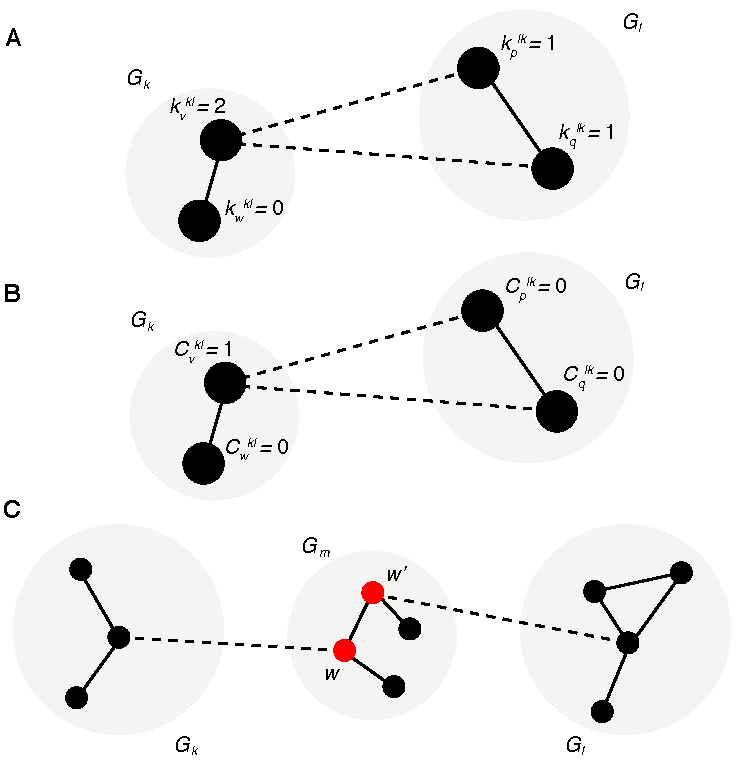
\includegraphics[width=\columnwidth]{cross_measures_schematic.pdf} 
\caption{Schematic illustration of some characteristics of interdependent networks: (A) The cross-degree $k_v^{kl}$ counts the number of neighbors of vertex $v\in V_k$ within the subnetwork $G_l$. In the example, the associated cross-edge density is $\rho_{kl}=0.5$. (B) The local cross-clustering coefficient $\mathcal{C}_v{kl}$ is the probability that two randomly drawn neighbors of vertex $v\in V_k$ from subnetwork $G_l$ are mutually connected. In the example, the associated global cross-clustering coefficients are given by $\mathcal{C}_{kl}=0.5$ and $\mathcal{C}_{lk}=0$, whereas the cross-transitivities are $\mathcal{T}_{kl}=1$ and $\mathcal{T}_{lk}=0$. (C) The cross-betweenness centrality $b_w^{kl}$ measures the fraction of shortest paths between vertices from subnetworks $G_k$ and $G_l$ that traverse vertex $w\in V_m$ (note that $G_m$ can coincide here with $G_k$ or $G_l$). In the example, $w,w'\in V_m$ (red) have a large cross-betweenness, whereas the remaining vertices $p\in V_m\setminus\{w,w'\}$ from subnetwork $G_m$ do not participate in shortest paths between $G_k$ and $G_l$ and therefore have vanishing cross-betweenness $b_p^{kl}=0$.}
\label{fig:interacting_measures}
\end{figure}

The \textit{cross-degree} (or \textit{cross-degree centrality})
\begin{equation}
\hat{k}_v^{kl} = \sum_{i \in V_l} A_{vi}
\label{eq:degree_cross}
\end{equation}
counts the number of neighbors of $v$ within $G_l$, i.e., direct connections between $G_k$ and $G_l$ (Fig.~\ref{fig:interacting_measures}A). Thus, this measure provides information on the relevance of $v$ for the network ``coupling'' between $G_k$ and $G_l$\footnote{In the specific case of an IRN, we interpret this as geometric signatures of the coupling between the underlying dynamical systems $X_k$ and $X_l$~\cite{Feldhoff2011,Feldhoff2012}.}. For the purpose of the present work, it is useful studying a normalized version of this measure, the \textit{cross-degree density}
\begin{equation}
\hat{\rho}_v^{kl} = \frac{1}{N_l} \sum_{i \in V_l} A_{vi} = \frac{1}{N_l} \hat{k}_v^{kl}.
\label{eq:locrho_cross}
\end{equation}
\noindent
For an IRN, $\hat{\rho}_v^{kl}(\varepsilon_{kl})$ equals the (cross-) recurrence rate $RR_{kl}(\varepsilon_{kl})$ (for $k=l$, it gives the corresponding single-system recurrence rate $RR_k(\varepsilon_k)$).

As for the single network case, important information is governed by the presence of triangles in the network. Given two subnetworks, the \textit{local cross-clustering coefficient}
\begin{equation}
\hat{\mathcal{C}}_v^{kl} = \frac{1}{\hat{k}_v^{kl}(\hat{k}_v^{kl} - 1)} \sum_{i,j \in V_l} A_{vi} A_{ij} A_{jv},
\label{eq:locclustering_cross}
\end{equation}
\noindent
measures the relative frequency of two randomly drawn neighbors $i,j\in V_l$ of $v\in V_k$ are mutually connected (Fig.~\ref{fig:interacting_measures}B). For $\hat{k}_v^{kl}<2$, we define $\hat{\mathcal{C}}_v^{kl}=0$. In general, $\hat{\mathcal{C}}_v^{kl}$ characterizes the tendency of vertices in $G_k$ to connect to clusters of vertices in $G_l$. 
%Unlike for the cross-degree, the standard local clustering coefficient does not directly follow by summing up the local cross-clustering coefficients of $v$ with respect to all subnetworks $G_l$, but requires more complex mathematical operations~\cite{Donges2011EPJB}. 

The \textit{cross-closeness centrality}
\begin{equation}
\hat{c}_v^{kl} = \left(\frac{\sum_{i \in V_l} d_{vi}}{N_l}\right)^{-1}
\label{eq:closeness_cross}
\end{equation}
\noindent
(where $d_{vi}$ is the graph-theoretical shortest-path length between $v$ and $i$) characterizes the topological closeness of $v\in G_k$ to $G_l$, i.e., the inverse arithmetic mean of the shortest path lengths between $v$ and all vertices $i\in V_l$. If there exist no such paths, $d_{vi}$ is commonly set to the maximum possible value $N-1$ given the size of $G$. As in the single network case, replacing the arithmetic by the harmonic mean yields the \textit{local cross-efficiency}
\begin{equation}
\hat{e}_v^{kl} = \frac{\sum_{i \in V_l} d_{vi}^{-1}}{N_l},
\label{eq:locefficiency_cross}
\end{equation}
\noindent
which can be interpreted in close analogy to $\hat{c}_v^{kl}$. Note that in the case of IRNs, topological closeness directly implies geometric closeness.

As a final vertex characteristic, we may generalize the betweenness concept to the case of coupled subnetworks, which results in the \textit{cross-betweenness centrality}
\begin{equation}
\hat{b}_v^{kl} = \sum_{i\in V_k,j\in V_l;i,j\neq v} \frac{\hat{\sigma}_{ij}(v)}{\hat{\sigma}_{ij}}.
\label{eq:betweenness_cross}
\end{equation}
\noindent
Here, $\hat{\sigma}_{ij}(v)$ and $\hat{\sigma}_{ij}$ are defined as in the case of a single network. Note that unlike the other vertex characteristics discussed above, in the case of cross-betweenness centrality, we do not require $v$ belonging to $G_k$ or $G_l$  (Fig.~\ref{fig:interacting_measures}C). The reason for this is that vertices belonging to any subnetwork may have a non-zero betweenness regarding two given subgraphs $G_k$ and $G_l$, in the sense that shortest paths between $i\in V_k$ and $j\in V_l$ can also include vertices in other subnetworks. 


\subsubsection{Global measures}

The density of connections between two subnetworks can be quantified by taking the arithmetic mean of the local cross-degree density (Eq.~\ref{eq:locrho_cross}), yielding the \textit{cross-edge density}
\begin{equation}
\hat{\rho}^{kl} = \frac{1}{N_k N_l} \sum_{i \in V_k, j \in V_l} A_{ij} = \hat{\rho}^{lk}.
\label{eq:globrho_cross}
\end{equation}
Notably, $\hat{\rho}^{kl}$ corresponds to the definition of the \textit{cross-recurrence rate} $RR_{kl}$ (Eq.~\ref{eq:crr}). Since we consider here only undirected networks (i.e., bidirectional edges), the cross-edge density is invariant under mutual exchange of the two considered subnetworks.

The \textit{global cross-clustering coefficient}
\begin{equation}
\hat{\mathcal{C}}^{kl} = \left<\hat{\mathcal{C}}_v^{kl}\right>_{v \in V_k} = \frac{1}{N_k} \sum_{v \in V_k, \hat{k}_v^{kl}>1} \frac{\sum_{i,j \in V_l} A_{vi} A_{ij} A_{jv}}{\sum_{i \neq j \in V_l} A_{vi} A_{vj}}
\label{eq:globclustering_cross}
\end{equation}
estimates the probability of vertices in $G_k$ to have mutually connected neighbors in $G_l$. Unlike the cross-edge density, the corresponding ``cross-transitivity'' structure is typically asymmetric, i.e., $\hat{\mathcal{C}}^{kl} \neq \hat{\mathcal{C}}^{lk}$. As in the single network case, we need to distinguish $\hat{\mathcal{C}}^{kl}$ from the \textit{cross-transitivity}
\begin{equation}
\hat{\mathcal{T}}^{kl} = \frac{\sum_{v \in V_k; i,j \in V_l} A_{vi} A_{ij} A_{jv}}{\sum_{v \in V_k; i \neq j \in V_l} A_{vi}  A_{vj}},
\label{eq:transitivity_cross}
\end{equation}
for which we generally have $\hat{\mathcal{T}}^{kl}(\varepsilon) \neq \hat{\mathcal{T}}^{lk}(\varepsilon)$ as well. Again, we have to underline that cross-transitivity and global cross-clustering coefficient are based on a similar concept, but capture distinctively different network properties.

Regarding the quantification of shortest path-based characteristics, we define the \textit{cross-average path length}
\begin{equation}
\hat{\mathcal{L}}^{kl} = \frac{1}{N_k N_l} \sum_{i \in V_k, j \in V_l} d_{ij} %= \hat{\mathcal{L}}_{lk}
\label{eq:apl_cross}
\end{equation}
and the \textit{global cross-efficiency}
\begin{equation}
\hat{\mathcal{E}}^{kl} = \left( \frac{1}{N_k N_l} \sum_{i \in V_k, j \in V_l} d_{ij}^{-1} \right)^{-1} %= \hat{\mathcal{E}}_{lk}.
\label{eq:globefficiency_cross}
\end{equation}
\noindent
Unlike $\hat{\mathcal{C}}^{kl}$ and $\hat{\mathcal{T}}^{kl}$, $\hat{\mathcal{L}}^{kl}$ and $\hat{\mathcal{E}}^{kl}$ are (as shortest path-based measures) symmetric by definition, i.e., $\hat{\mathcal{L}}^{kl}(\varepsilon)=\hat{\mathcal{L}}^{lk}(\varepsilon)$ and $\hat{\mathcal{E}}^{kl}(\varepsilon)=\hat{\mathcal{E}}^{lk}(\varepsilon)$. In the case of disconnected network components, the shortest path length $d_{ij}$ is defined as discussed for the corresponding local measures.

%All aforementioned global characteristics quantify certain aspects of the interdependence structure between two subnetworks and can be derived from contributions of local (single-vertex) measures. Notably, we may also proceed in a similar way regarding the cross-betweenness centrality to obtain a \textit{global cross-betweenness} by setting
%\begin{equation}
%\hat{\mathcal{B}}_{kl}=\frac{1}{K}\sum_{m=1}^K \hat{\mathcal{B}}^{kl|m}
%\end{equation}
%\noindent
%with
%\begin{equation}
%\hat{\mathcal{B}}_{kl|m} = \frac{1}{N_m} \sum_{v\in V_m} \hat{b}_{v}^{kl}.
%\end{equation}
%\noindent
%We note that using betweenness as a global network characteristics is quite uncommon in complex network theory, so that we will not further utilize this measure here. Specifically, $\hat{\mathcal{B}}_{kl}$ quantifies the total number of shortest paths between elements from $G_k$ and $G_l$, including both direct connections (which have already been characterized by the cross-edge density) and indirect connections (i.e., shortest paths traversing further vertices within $G_k$ and $G_l$ or even other subnetworks). Regarding the latter aspect, consideration of $\hat{\mathcal{B}}_{kl|m}$ connecting three subnetworks might be particularly interesting. Here, we expect $\hat{\mathcal{B}}_{kl|m}=\hat{\mathcal{B}}_{lk|m}$, but $\hat{\mathcal{B}}_{kl|m}\neq \hat{\mathcal{B}}_{km|l}$ etc. In this spirit, $\hat{\mathcal{B}}_{kl|m}$ can be interpreted as a \emph{conditional} global network characteristics.

In the same spirit as shown above, other single network characteristics~\cite{Boccaletti2006,Costa2007} can be adopted as well for defining further interdependent network measures. This includes measures characterizing edges or, more generally, pairs of vertices like edge betweenness or matching index, further global network characteristics (assortativity, network diameter and radius), mesoscopic structures (motifs), or even characteristics associated with diffusion processes on the network instead of shortest paths (e.g., eigenvector centrality or random walk betweenness). The selection of measures introduced above reflects those characteristics which have the most direct interpretation in the context of IRNs and have also been utilized in studying the interdependence structure between complex networks in other contexts~\cite{Donges2011EPJB,Wiedermann2013}. %A more detailed discussion of further measures, including the derivation of closed-form expressions and possible continuous generalizations (see Section~\ref{sec:analytics}) is left as a topic of future research.


\subsection{Joint recurrence networks}\label{sec:jrn}

\subsubsection{Basic idea}\label{sec:jrn_classic}

Besides cross-recurrences, another possible multivariate generalization of RPs is studying joint recurrences of different systems in their individual (possibly different) phase spaces. Here, the basic idea is that the simultaneous occurrence of recurrences in two or more systems $\{X_k\}$ (see Fig.~\ref{fig:sketch_cr_jr}) contains information on possible interrelationships between their respective dynamics, for example, the emergence of generalized synchronization~\cite{Romano2004PLA,Romano2005EPL}. Consequently, based on time series $\{x_i^k\}$, the joint recurrence matrix $\mathbf{JR}$ with elements
\begin{equation}
JR_{ij}(\varepsilon_1,\dots,\varepsilon_K)=\prod_{k=1}^K R_{ij}^k(\varepsilon_k)
\end{equation}
is defined as the element-wise product of the single-system recurrence matrices $\mathbf{R}^k$ with elements
\begin{equation}
R_{ij}^k(\varepsilon_k)=\Theta(\varepsilon_k - \|x_i^k - x_j^k\|), 
\end{equation}
where $(\varepsilon_1,\dots,\varepsilon_K)$ is the vector of recurrence thresholds that can be selected for each time series individually, typically such as to yield the same global recurrence rates $RR_k=RR$ for all $k=1,\dots,K$.

Analogously to single-system recurrence network analysis, we can take a graph-theoretical perspective by defining a \emph{joint recurrence network (JRN)} by its adjacency matrix
\begin{equation}
\mathbf{A}(\varepsilon_1,\dots,\varepsilon_K) = \mathbf{JR}(\varepsilon_1,\dots,\varepsilon_K) - \mathbf{1}_N,
\end{equation}
where $\mathbf{1}_N$ again denotes the $N$-dimensional identity matrix. Hence, edges $(i,j)$ of a JRN indicate joint recurrences occurring simultaneously in \emph{all} $K$ time series under study. Alternatively, $\mathbf{A}(\varepsilon_1,\dots,\varepsilon_K)$ may be viewed as the element-wise product of the single-system recurrence networks' adjacency matrices $\mathbf{A}^k(\varepsilon_k)$.

As single-system RN and IRN, the JRN describes an undirected and unweighted simple graph. However, due to the temporal simultaneity condition of the joint recurrence concept, vertices $i$ are explicitly associated with points in time $t^k_i=t^l_i$ common to the $K$ considered time series (cf.~Tab.~\ref{tab:multivariate_rns}). This is conceptually different from RNs and IRNs where time information is not taken into account so that network characteristics are invariant under permutations of the state vectors (i.e., the -- possibily embedded -- observations). More specifically, it is not possible to relabel the observations in the underlying time series prior to the computation of the JRN, whereas the JRN vertices can be shuffled again without altering the resulting network properties. 

By construction, the time series $\{x_i^k\}$ used for constructing a JRN need to be sampled at identical times $\{t^k_i\}$ and have to have the same length, \textit{i.e.}, $N_1=N_2=\dots=N_K=N$. However, since recurrences are compared instead of state vectors, the $\{x_i^k\}$ neither have to represent the same physical quantity measured in identical units, nor need they reside in the same phase space (Tab.~\ref{tab:multivariate_rns}). 

From a conceptual perspective, a JRN can be regarded as a simple RN for the combined system $(X_1\otimes\cdots\otimes X_K)$ in its higher-dimensional phase space spanned by all state variables. However, recurrences are defined here in some non-standard way taking distances in the subspaces associated with the individual systems separately into account. This implies that the properties of JRNs can be studied in essentially the same way as those of single-system RNs (but with possibly more subtle geometric interpretations of the respective network characteristics). In turn, comparing the same properties for JRN and single-system RNs provides important information about the similarity of neighborhood relationships in the combined phase space and projections on the individual systems' subspaces. Specifically, we can gain insights about the effective degrees of freedom of the combined system, which may be reduced in comparison with the sum of the degrees of freedom of the uncoupled systems due to dynamical interdependences between its components. We will further detail this idea in Section~\ref{sec:sync}.


\subsubsection{$\alpha$-joint recurrence networks}\label{sec:jrn_alpha}

Equivalently to their interpretation outlined in Section~\ref{sec:jrn_classic}, we can also consider JRNs as the reduction of a generalized graph, where the vertices correspond to time points $t_i$, which can be connected by at most $K$ different types of (labelled) edges representing the mutual closeness of states in the $K$ different systems. In this viewpoint, the reduction towards the JRN follows from the requirement that for a given pair of vertices, in the generalised graph \emph{all} $K$ possible labelled edges must be present. With other words, in terms of Boolean logics the entries of the binary recurrence matrices $\mathbf{R}^k$ are connected by a logical AND for defining the elements of $\mathbf{JR}$.

Notably, the presence of a joint recurrence becomes increasingly unlikely as the number of possibly interacting systems $K$ increases. Even in the case of very strong interdependences, there may be stochastic fluctuations in the individual systems (e.g., observational noise) that mask recurrences in individual systems and, thus, subsequently reduce the \emph{joint recurrence rate}
\begin{equation}
JRR(\varepsilon_1,\dots,\varepsilon_K) = \frac{2}{N(N-1)} \sum_{i=1}^{N-1} \sum_{j=i+1}^N JR_{ij} (\varepsilon_1,\dots,\varepsilon_K)
\end{equation}
\noindent
aka JRN edge density $\rho_J$.

One possibility to circumvent the problem sketched above is relaxing the requirement of having simultaneous recurrences in all systems (i.e., the logical AND operation connecting the recurrence matrices of the individual systems in a component-wise way), but considering the case where at least a fraction $\alpha\in(0,1]$ of all systems exhibit recurrences (the standard JRN follows for $\alpha=1$). This point of view allows defining a hierarchy of networks, which we call \textit{$\alpha$-joint recurrence networks ($\alpha$-JRN)}. Starting from the union of the single-system RNs providing a network with $K$ different edge types corresponding to recurrences of the individual systems, we require that there exist at least $\lceil\alpha K\rceil$ edges between two specified vertices (i.e., time points). In the specific case of $K=2$ systems and $\alpha\in(0,0.5]$ (or, more generally, for $\alpha\in(0,1/K]$), we can rewrite this requirement with a simple logical (Boolean) operation connecting the single-system recurrence matrices in a component-wise way as $JR^{\alpha}_{ij}(\varepsilon_1,\varepsilon_2) = R^{X_1}_{ij}(\varepsilon_1)\ \mbox{OR}\ R^{X_2}_{ij}(\varepsilon_2)$.

For the more general case, in order to mathematically formulate the requirement of $\lceil\alpha K\rceil$ simultaneous recurrences, it is convenient to start from a practically equivalent re-definition of the joint recurrence matrix,
\begin{equation}
JR^*_{ij}(\varepsilon_1,\dots,\varepsilon_K) = \Theta\left( \sum_{k=1}^K R_{ij}^k(\varepsilon_k) -K-\delta \right),
\end{equation}
\noindent
with the usual Heaviside function $\Theta(\cdot)$ and $\delta\to 0^+$ being infinitesimally small (to assure $JR^*_{ij}=1$ if $\sum_{k=1}^K R_{ij}^k=K$), and set
\begin{equation}
JR^{\alpha}_{ij}(\varepsilon_1,\dots,\varepsilon_K) = \Theta\left( \sum_{k=1}^K R_{ij}^k(\varepsilon_k) -\alpha K-\delta \right),
\end{equation}
\noindent
to be the \emph{$\alpha$-joint recurrence matrix}. We can use the latter definition to define $\alpha$-joint recurrence plots as well as $\alpha$-JRNs in full analogy to the classical case $\alpha=1$.

Trivially, the number of edges in an $\alpha$-JRN decreases monotonically for increasing $\alpha$ if all single-system recurrence thresholds $\varepsilon_k$ are kept fixed. We note that a similar relaxation of the strict requirement of a conjection (AND relation) between the (Boolean) entries of different recurrence matrices has been recently discussed in the framework of symbolic recurrence plots~\cite{Donner2008}. Moreover, it might be interesting (but has not yet been explored) to use concepts from fuzzy logic as the basis for somewhat weaker requirements than in the rather restrictive definition of the original JRN.

The conceptual idea of $\alpha$-JRNs has not yet been further developed and studied elsewhere. One possible field of application could be finding proper values of $\alpha$ (for example, in dependence on the magnitude of some observational noise) for which results commonly obtained using ``normal'' JRNs become stable in the case of real-world time series. To this end, we only emphasize the possibility of defining $\alpha$-JRNs and studying the properties of these entities (e.g., the scaling of network characteristics as a function of $\alpha$), but leave a corresponding investigation as a subject for future research.

%\subsection{{\color{red}short subsection on MRPs and possible network interpretation???}}

%\subsection{{\color{red}Practical considerations: How to fix (cross-) edge densities?}}


\section{Analytical description of recurrence networks}\label{sec:analytics}

As we will demonstrate in the following, the properties of RNs can be described analytically supporting their better understanding and, hence, applicability. For this purpose, we can exploit the formal equivalence of RNs and random geometric graphs (RGGs), a well-studied concept in graph theory and computational geometry. In this section, we motivate this equivalence and demonstrate how the variety of RN characteristics can be reformulated in the continuum limit $N\to\infty$ for any finite $\varepsilon$. This framework allows gaining deep insights into the geometric organization of chaotic attractors by exploring the multitude of characteristics provided by complex network theory. Moreover, we present a first-time extension~\cite{Donges2012PhD} of the previous analytical considerations \cite{Donges2012PRE} to IRNs.


\subsection{Random geometric graphs}

Random geometric graphs \cite{Penrose2003} are based on a (finite) set of vertices randomly positioned in a $d$-dimensional ($d\in\mathbb{N}^+$) metric space according to some probability density function $p(x)$. In general, the connectivity among this set of vertices is taken to be distance-dependent, i.e., for two vertices $i$ and $j$, the probability of being connected in the RGG has the form $P(A_{ij}=1)=f(\|x_i-x_j\|)$ with some predefined function $f$, which is monotonically decreasing. As a consequence, spatially close vertices are more likely to be connected than distant ones. A particularly well studied special case is $f(\delta)=\Theta(\varepsilon-\delta)$ ($\delta$ denoting here the distance between any two points in the considered metric space), often refered to as RGG (in the strict sense). Notably, the latter definition has fundamental real-world importance (e.g., in terms of ad-hoc communication networks or, more general, contact networks) and matches that of the adjacency matrix of a RN (Eq.~\ref{eq:rn_definition}) if we identify $p(x)$ with the invariant density of the dynamically invariant object under study (e.g., some attractor in case of a dissipative system), and take the space in which the RGG is embedded as that spanned by the respective dynamical variables of the system. In this respect, for all following considerations, it is sufficient restricting attention to the support of $p(x)$ (respectively its closure), which is described by some manifold $S=\overline{\mbox{supp}(p)}$ embedded in the considered metric space (e.g., the attractor manifold).

\begin{figure}
\centering
\resizebox{0.475\textwidth}{!}{\includegraphics*{roessler_attractor_rgg_N_10.pdf}} \hfill
\resizebox{0.475\textwidth}{!}{\includegraphics*{roessler_attractor_rgg_N_100.pdf}} \\
\resizebox{0.475\textwidth}{!}{\includegraphics*{roessler_attractor_rgg_N_500.pdf}} \hfill
\resizebox{0.475\textwidth}{!}{\includegraphics*{roessler_attractor_rgg_N_1000.pdf}}
\caption{Example of RGGs constructed from the invariant density of the R\"ossler system (Eq.~\ref{eq:roessler}) using sample sizes of $N=10$, $100$, $500$ and $1000$ and a fixed $\varepsilon=2.0$. In order to obtain a better visualization, only projections of the attractor and resulting graph to the $(x,y)$-plane are shown. Note that although the attractor's invariant density is not yet well sampled at $N=1,000$, most network characteristics obtained from the corresponding RN (not shown) already provide reasonable approximations of the expected values for the underlying RGG.}
\label{fig:roessler_rgg}
\end{figure}

Figure~\ref{fig:roessler_rgg} shows some example of RGGs obtained using the invariant density of the R\"ossler system (Eq.~\ref{eq:roessler}) as $p(x)$. Specifically, the RGG has been obtained from the numerical realization of a single trajectory of the system, which has been downsampled to a certain fixed sampling rate. 

From a practical perspective, the spatial coverage of $p(x)$ by the RGG's vertices can be strongly affected by the sampling, leading to a spatial clustering of vertices if the sampling frequency is close to an integer multiple of the chaotic attractor's characteristic frequency. In such a situation, it is advantageous to follow alternative sampling strategies for $p(x)$\footnote{For ergodic systems, sampling from one long trajectory, ensembles of short independent realizations of the same system, or directly from the invariant density should lead to networks with the same properties at sufficiently large $N$.}. As already mentioned above, generating the RGG/RN representation based on bootstrapping from the ensemble of available state vectors is superior to a regular sampling of a given trajectory.

As outlined above, the importance of RGGs for the considerations on RNs is that some of their properties (like the degree distribution~\cite{Herrmann2003} or transitivity~\cite{Dall2002}) have been intensively studied in the past for the generic case of a hard distance threshold in $f$ and arbitrary probability density functions $p(x)$ for metric spaces of various integer dimensions. For example, Hermann \textit{et~al.} \cite{Herrmann2003} give a closed-form expression of the degree distribution for arbitrary $p(x)$, whereas Dall and Christensen~\cite{Dall2002} provide a deep discussion of the transitivity properties of RGGs. Notably, the latter aspect has become particularly relevant in the interpretation of RN properties as well as their multivariate generalizations, as will be further discussed in Section~\ref{sec:rn_properties}.


\subsection{Single-system recurrence network characteristics}\label{sec:rn_theory}

By making use of the fact that RNs are a specific type of RGGs, all relevant graph-theoretical measures for recurrence networks can be seen as discrete approximations of more general and continuous geometrical properties of a dynamical system's underlying attractor characterized by a set $S$ together with an associated invariant density $p(x)$, $x\in S$. This point of view allows obtaining deeper insights into the geometrical meaning of the network quantifiers introduced in Section~\ref{sec:rn_measures} and enables us to establish surprising connections to other fields, \textit{e.g.}, the close relationship of transitivity measures like the local clustering coefficient and transitivity to the local and global fractal dimension of the dynamical system's attractor, respectively~\cite{Donner2011EPJB}, see Section~\ref{sec:transitivity}. In the following, we review a corresponding analytical framework for general spatially embedded networks which is specifically tailored for defining continuous variants of the common discrete complex network characteristics \cite{Donges2012PRE}.


\subsubsection{General setting}

Let $S$ be a compact and smooth manifold with a non-vanishing continuous probability density function $p:S\to(0,\infty)$ with $\int_S dx\ p(x) = 1$. For the purpose of the present work, we identify $S$ with the set of points defining the attractor of a (dissipative) dynamical system. In case of chaotic attractors in time-continuous systems, we obtain a closure of the open attractive set by considering its union with the set of (infinitely many) unstable periodic orbits embedded in the attractor.

Continuous analogs of the discrete complex network characteristics introduced in Section~\ref{sec:rn_measures} should be approximated by taking the limit $N\to\infty$ and $\varepsilon\to 0$ (note that the latter limit may not be assessible in the case of fractal sets $S$, which we will not further consider in the following). Here, ``continuous'' refers to a network with uncountably many vertices and edges, which is determined by the \emph{adjacency function}
\begin{equation}
A(x,y)=\Theta(\varepsilon-\|x-y\|)-\delta(x-y)
\end{equation}
\noindent
for all $x,y\in S$, which is a continuous analog of the adjacency matrix. In the latter expression, $\delta(x-y)=1$ if $x=y$, and $0$ otherwise.


\subsubsection{Shortest paths and geodesics}

A large variety of complex network characteristics introduced in Section~\ref{sec:rn_measures} relies on the concept of shortest paths. Examples include closeness and betweenness centrality, local and global efficiency, and average path length. In the continuum limit, we consider a path in $S$ as a closed curve described by a properly parametrized function $f:[0,1]\to S$, and define the associated path length 
\begin{equation}
l(f) = \sup_{n>0; \{t_i\}_{i=1}^n} \left.\left\{ \sum_{i=1}^n d(f(t_{i-1}),f(t_i)) \right| 0=t_0\leq t_1\leq\dots\leq t_n=1 \right\} \in[0,\infty] 
%{n>0,\\0=t_0\leq t_1\leq\dots\leq t_n=1} \sum_{i=1}^n d(f(t_{i-1}),f(t_i)),
\end{equation}
\noindent
%$l(f)\in[0,\infty]$ as the supremum of $\sum_{i=1}^n d(f(t_{i-1}),f(t_i))$ over all $n>0$ and $0=t_0\leq t_1\leq\dots\leq t_n=1$, 
where $d(\cdot)$ denotes some metric used for defining distances on $S$. The \textit{geodesic distance} between two points $x,y\in S$, which serves as the analog of the shortest path length on a network, is then defined as (cf.~Fig.~\ref{fig:manifold}).
\begin{equation}
g(x,y) = \inf_f \left\{ l(f)\ |\ f:[0,1]\to S,\ f(0)=x,\ f(1)=y \right\}.
\end{equation}
\noindent
A path of length $g(x,y)$ is called a \emph{global geodesic} on $S$. Depending on the specific geometry of the considered set $S$, the multiplicity of global geodesics connecting $x$ and $y$ may differ, including no, one, or even infinitely many distinct global geodesics.

\begin{figure}
\centering
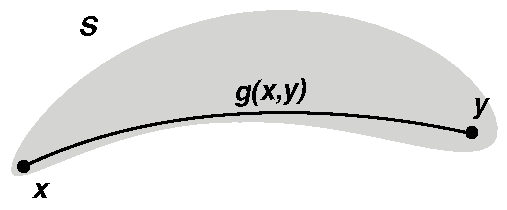
\includegraphics[width=.50\columnwidth]{fig1.pdf} 
\caption{Schematic illustration of a set $S$ (gray), where $g(x,y)$ denotes the geodesic distance between $x,y\in S$ (after \cite{Donges2012PRE}).}
\label{fig:manifold}
\end{figure}

Regarding a continuum limit for RNs, we note that shortest paths in such networks approximate global geodesics on the underlying invariant set $S$ in the limit of $\varepsilon\to 0$ and $N\to\infty$. Specifically, in the latter limit the shortest path length $l_{ij}(\varepsilon)$ between two points $x(t_i), x(t_j)\in S$ behaves as
\begin{equation}
\varepsilon\ l_{ij}(\varepsilon) \to g(x(t_i),x(t_j))
\end{equation}
\noindent 
independently of the chosen metric~\cite{Donges2012PRE}.

For defining betweenness centrality, we do not only require information on the lengths of global geodesics, but also their total multiplicity $\sigma(y,z;\varepsilon)$ as well as their multiplicity conditional on a third point $x\in S$ being part of the curve, denoted as $\sigma(y,z|x;\varepsilon)$ in the following. The definition of the latter quantity is, however, not unique for a given finite $\varepsilon$. Two possible, yet generally not equivalent expressions read~\cite{Donges2012PRE}
\begin{eqnarray}
\sigma_1(y,z|x;\varepsilon) &=& \sum_{k=1}^{\sigma(y,z;\varepsilon)} \int_0^1 dt\ \delta(f_k(t)-x) \label{eq:nrpaths_cont1} \\
\sigma_2(y,z|x;\varepsilon) &=& \sum_{k=1}^{\sigma(y,z;\varepsilon)} \int_0^1 dt\ \Theta(\varepsilon-\|f_k(t)-x\|), \label{eq:nrpaths_cont2}
\end{eqnarray}
\noindent
where $f_k(t)$ denotes the family of global geodesics between $y$ and $z$. Note that this family can have uncountably many members (to see this, consider, for example, the set of geodesics between the two poles on a sphere). In this case, the sum in Eqs.~(\ref{eq:nrpaths_cont1}) and (\ref{eq:nrpaths_cont2}) should be replaced by an integral. Furthermore, we emphasize that the $\varepsilon$-dependence in the multiplicities of shortest paths is implicit rather than explicit, since the chosen discretization level $\varepsilon$ can affect the effective ``shape'' of $S$ and, hence, the positions of possible edges in the considered space.


\subsubsection{Local (vertex-based) measures}

The \emph{continuous $\varepsilon$-degree density}
\begin{equation}
\rho(x;\varepsilon)=\int_{B_{\varepsilon}(x)} d\mu(y)
\end{equation}
\noindent
gives the probability that a point $y\in S$ randomly drawn according to $p$ falls into an $\varepsilon$-neighborhood $B_{\varepsilon}(x)=\{y\in S\,|\, \|x-y\|<\varepsilon\}$ around $x$. Its discrete estimator is given by the classical degree density $\hat{\rho}_v(\varepsilon)$ (Eq.~\ref{eq:locrho}).

In order to quantify the density of closed paths of length 3 in the network, we can consider the \emph{continuous local $\varepsilon$-clustering coefficient}
\begin{equation}
\mathcal{C}(x;\varepsilon)=\frac{\int\int_{B_{\varepsilon}(x)} d\mu(y)\ d\mu(z)\ \Theta(\varepsilon-\|y-z\|)}{\rho(x;\varepsilon)^2}.
\end{equation}
\noindent
This measure characterizes the probability that two points $y$ and $z$ randomly drawn according to $p$ from the $\varepsilon$-neighborhood of $x\in S$ are mutually closer than $\varepsilon$. Its discrete approximation is provided by the classical local clustering coefficient $\hat{\mathcal{C}}_v(\varepsilon)$ (Eq.~\ref{eq:locclustering}).

Let $y\in S$ be drawn randomly according to $p$. For a fixed $x\in S$, the \emph{continuous $\varepsilon$-closeness centrality}
\begin{equation}
c(x;\varepsilon)=\left(\int_S d\mu(y)\ \frac{g(x,y)}{\varepsilon}\right)^{-1}
\end{equation}
\noindent
and the \emph{continuous local $\varepsilon$-efficiency} 
\begin{equation}
e(x;\varepsilon)=\int_S d\mu(y)\ \left(\frac{g(x,y)}{\varepsilon}\right)^{-1}
\end{equation}
\noindent
give the inverse expected geodesic distance and the expected inverse geodesic distance of $y$ to $x$, respectively. Hence, both measures quantify the geometric closeness of $x$ to any other point in $S$ according to the probability density function $p$. By making use of RNs, they can be approximated by the classical closeness centrality $\hat{c}_v(\varepsilon)$ (Eq.~\ref{eq:closeness}) and local efficiency $\hat{e}_v(\varepsilon)$ (Eq.~\ref{eq:locefficiency}).

Finally, the probability that a point $x$ lies on a randomly chosen global geodesic connecting two points $y,z\in S$ according to $p$ is measured by the \emph{continuous $\varepsilon$-betweenness centrality}
\begin{equation}
b(x;\varepsilon)=\int\int_S d\mu(y)\ d\mu(z)\ \frac{\sigma(y,z|x;\varepsilon)}{\sigma(y,z;\varepsilon)}.
\end{equation}
\noindent
Its discrete estimator is given by the standard RN betweenness centrality $\hat{b}_v(\varepsilon)$ (Eq.~\ref{eq:betweenness}) with the different possible expressions for $\sigma(y,z|x;\varepsilon)$ (Eqs.~\ref{eq:nrpaths_cont1},\ref{eq:nrpaths_cont2}) \cite{Donges2012PRE}.


\subsubsection{Pairwise vertex and edge measures}

The \emph{continuous $\varepsilon$-matching index}
\begin{equation}
m(x,y;\varepsilon)=\frac{\int_{B_{\varepsilon}(x)\cap B_{\varepsilon}(y)}d\mu(z)}{\int_{B_{\varepsilon}(x)\cup B_{\varepsilon}(y)}d\mu(z)}
\end{equation}
\noindent
quantifies the mutual overlap between the neighborhoods of two vertices $x,y\in S$. In other words, $m(x,y;\varepsilon)$ is the probability that a point $z\in S$ randomly chosen from $B_{\varepsilon}(x)$ according to $p$ is also contained in $B_{\varepsilon}(y)$ and vice versa. For $x\to y$, we have $B_{\varepsilon}(x)\to B_{\varepsilon}(y)$ and, consequently, $m(x,y;\varepsilon)\to 1$, whereas $m(x,y;\varepsilon)=0$ if $\|x-y\|>2\varepsilon$. As in the case of the other measures described above, $m(x,y;\varepsilon)$ can be approximated by the discrete RN matching index $\hat{m}_{vw}(\varepsilon)$ (Eq.~\ref{eq:matching}).

$m(x,y;\varepsilon)$ does not require mutual closeness between $x$ and $y$ (i.e., $\|x-y\|\in(\varepsilon,2\varepsilon)$ is possible). In contrast, the \emph{continuous $\varepsilon$-edge betweenness}
\begin{equation}
b(x,y;\varepsilon)=\int\int_S d\mu(z)\ d\mu(z')\ \frac{\sigma(z,z'|x,y;\varepsilon)}{\sigma(z,z';\varepsilon)}
\end{equation}
\noindent
(with $\sigma(z,z'|x,y;\varepsilon)$ denoting the number of global geodesics between $z$ and $z'$ containing both $x$ and $y$ under the condition $\|x-y\|\leq\varepsilon$, and $\sigma(z,z';\varepsilon)$ the total number of global geodesics between $z$ and $z'$) is a measure whose discrete estimator $\hat{b}_{vw}(\varepsilon)$ (Eq.~\ref{eq:edgebetweenness}) is related to the presence of an edge between $x(t_v)$ and $x(t_w)$, i.e., $\|x(t_v)-x(t_w)\|< \varepsilon$. However, although this property has been originally introduced as an explicit edge property, it can be understood in a more general way as a two-vertex property such that $b(x,y;\varepsilon)$ measures the probability that two specific (not necessarily $\varepsilon$-close) points $x$ and $y$ both lie on a $p$-randomly drawn global geodesic connecting two points $z,z'\in S$ \emph{and} are mutually closer than $\varepsilon$. Further generalizations towards $n$-point relationships are possible, but not instructive within the scope of this work.


\subsubsection{Global network measures}

The \emph{continuous $\varepsilon$-edge density}
\begin{equation}
\rho(\varepsilon)=\int_S d\mu(x)\ \rho(x;\varepsilon)
\end{equation}
\noindent
is the $p$-expectation value of the continuous $\varepsilon$-degree density and approximated by the discrete edge density $\hat{\rho}(\varepsilon)$ of a RN (Eq.~\ref{eq:edgedensity}).

In the same spirit, the \emph{continuous global $\varepsilon$-clustering coefficient}
\begin{equation}
\mathcal{C}(\varepsilon)=\int_S d\mu(x)\ \mathcal{C}(x;\varepsilon)
\end{equation}
\noindent
is the $p$-expectation value of the continuous local $\varepsilon$-clustering coefficient. Its associated discrete estimator is the classical global (Watts-Strogatz) clustering coefficient $\hat{\mathcal{C}}(\varepsilon)$ (Eq.~\ref{eq:globclustering}). As an alternative measure characterizing geometric transitivity, we can define the \emph{continuous $\varepsilon$-transitivity}
\begin{equation}
\mathcal{T}(\varepsilon)=\frac{\int\int\int_S d\mu(x)\, d\mu(y)\, d\mu(z)\, \Theta(\varepsilon-\|x-y\|)\, \Theta(\varepsilon-\|y-z\|)\, \Theta(\varepsilon-\|z-x\|)}{\int\int\int_S d\mu(x)\, d\mu(y)\, d\mu(z)\, \Theta(\varepsilon-\|x-y\|)\, \Theta(\varepsilon-\|z-x\|)},
\end{equation}
\noindent
which gives the probability that among three points $x,y,z\in S$ randomly drawn according to $p$, $y$ and $z$ are mutually closer than $\varepsilon$ given they are both closer than $\varepsilon$ to $x$. The corresponding discrete estimator is the RN transitivity $\hat{\mathcal{T}}(\varepsilon)$ (Eq.~\ref{eq:transitivity}).

As examples of shortest path-based characteristics, we can define the \emph{continuous $\varepsilon$-average path length}
\begin{equation}
\mathcal{L}(\varepsilon)=\int\int_S d\mu(x)\ d\mu(y)\ \frac{g(x,y)}{\varepsilon}
\end{equation}
\noindent
and the \emph{continous global $\varepsilon$-efficiency}
\begin{equation}
\mathcal{E}(\varepsilon)=\left(\int\int_S d\mu(x)\ d\mu(y)\ \left(\frac{g(x,y)}{\varepsilon}\right)^{-1}\right)^{-1},
\end{equation}
\noindent
which measure the expected geodesic distance and the inverse of the expected inverse geodesic distance, respectively, both measured in units of $\varepsilon$ between two points $x,y\in S$ drawn randomly according to $p$. Their discrete estimators are given by the classical RN average path length $\hat{\mathcal{L}}(\varepsilon)$ (Eq.~\ref{eq:apl}) and global efficiency $\hat{\mathcal{E}}(\varepsilon)$ (Eq.~\ref{eq:globefficiency}), respectively. Notably, we can reformulate $\mathcal{L}(\varepsilon)$ as the $p$-expectation value of the inverse continuous $\varepsilon$-closeness centrality,
\begin{equation}
\mathcal{L}(\varepsilon)=\int_S d\mu(x)\ c(x;\varepsilon)^{-1},
\end{equation}
\noindent
and $\mathcal{E}(\varepsilon)$ the inverse $p$-expectation value of the continuous local $\varepsilon$-efficiency
\begin{equation}
\mathcal{E}(\varepsilon)=\left(\int_S d\mu(x)\ e(x;\varepsilon)\right)^{-1}.
\end{equation}


\subsubsection{Further characteristics}

The selection of measures discussed above is far from being complete. Continuous versions of further complex network characteristics, such as assortativity, network diameter and radius, and network motifs are discussed in \cite{Donges2012PRE}, where also some outlook on corresponding generalizations of other measures like eigenvector centrality or random walk betweenness has been given. To this end, we restrict ourselves to the measures discussed above, since they have been most commonly used in recent applications of the RN framework.


\subsection{Inter-system recurrence network characteristics}\label{sec:irn_theory}

In the same spirit as for the single-system RNs (Section~\ref{sec:rn_theory}), we can consider the graph-theoretical measures for studying the interconnections between subnetworks within IRNs (Section~\ref{sec:irn_measures}) as discrete approximations of more general geometric properties \cite{Donges2012PhD}. Let $S_k \subset Y$ be a subset of an $m$-dimensional compact smooth manifold $Y$ and $p_k(x)$ represent its invariant density for all $k=1,\dots,K$, where $x\in S_k$. In the following, the $S_k$ and $p_k$ are assumed to fulfill the same requirements that are stated for $S$ and $p$ in Section~\ref{sec:rn_theory}. Notably, the $S_k$ are assumed to have a considerable non-empty pairwise intersections. We will use the abbreviation $\int d\mu_k(x)=\int_{S_k} d^mx\,p_k(x)$, where $\mu_k$ is a probability measure on $S_k$. For simplicity, only a single recurrence threshold $\varepsilon=\varepsilon_{kl}$ for all $k,l$ will be used in the following. The generalization to different values of $\varepsilon_{kl}$ is straightforward.

%In all definitions made below, $x$ denotes a state of system $X_k$, hence, $x \in S_k$ holds.


\subsubsection{Local measures}

The \emph{continuous $\varepsilon$-cross-degree density}
\begin{equation}
\rho^{kl}(x;\varepsilon) = \int_{B_\varepsilon(x) \cap S_l} d\mu_l(y) = \int d\mu_l(y) \Theta(\varepsilon - \|x-y\|)
\end{equation}
\noindent
measures the probability that a randomly chosen point in $S_l$ is found in the neighborhood $B_\varepsilon(x)$ of $x\in S_k$. Its discrete version is the cross-degree density $\hat{\rho}_v^{kl}(\varepsilon)$ (Eq.~\ref{eq:locrho_cross}).

The \emph{continuous local $\varepsilon$-cross-clustering coefficient}
\begin{equation}
\mathcal{C}^{kl}(x;\varepsilon) = \frac{\int\!\!\!\int_{B_\varepsilon(x) \cap S_l} \,d\mu_l(y)\,d\mu_l(z)\, \Theta(\varepsilon-\|y-z\|)}{\rho^{kl}(x;\varepsilon)^2}
\end{equation}
gives the probability that two randomly chosen points $y,z\in S_l$ are $\varepsilon$-close to each other ($\|y-z\|<\varepsilon$) if they both lie in the neighborhood of $x\in S_k$. $\mathcal{C}^{kl}(x;\varepsilon)$ is approximated by the discrete local cross-clustering coefficient $\hat{\mathcal{C}}_v^{kl}(\varepsilon)$ (Eq.~\ref{eq:locclustering_cross}).

Considering the mutual global geometry of the sets $S_k,S_l$, we furthermore introduce \textit{continuous $\varepsilon$-cross-closeness centrality}
\begin{equation}
c^{kl}(x;\varepsilon) = \left( \int d\mu_l(y) \, \frac{g(x,y)}{\varepsilon} \right)^{-1}
\end{equation}
quantifying the closeness of $x\in S_k$ to all points of the set $S_l$ along geodesics together with the related harmonic \textit{continuous local $\varepsilon$-cross-efficiency}
\begin{equation}
e^{kl}(x;\varepsilon) = \int d\mu_l(y) \, \left( \frac{g(x,y)}{\varepsilon} \right)^{-1}.
\end{equation}
Here, geodesics are defined with respect to the union of all involved systems' attractors $S=\bigcup_{k=1}^K S_k$ and $g(x,y)$ is a suitable distance metric on such geodesics (Section~\ref{sec:rn_theory}). The proposed local path-based measures for interdependent networks are approximated by the discrete cross-closeness centrality $\hat{c}_v^{kl}(\varepsilon)$ (Eq.~\ref{eq:closeness_cross}) and local cross-efficiency $\hat{e}_v^{kl}(\varepsilon)$ (Eq.~\ref{eq:locefficiency_cross}). 

Finally, we define the \textit{continuous $\varepsilon$-cross-betweenness centrality}
\begin{equation}
b^{kl}(x;\varepsilon)=\int \int d\mu_k(y)\ d\mu_l(z)\ \frac{\sigma(y,z|x;\varepsilon)}{\sigma(y,z;\varepsilon)}.
\end{equation}
\noindent
As in the single network case, $\sigma(y,z|x;\varepsilon)$ denotes the number of times $x\in S$ (i.e., from any arbitrary subnetwork) lies on a geodesic between $y\in S_k$ and $z\in S_l$, and $\sigma(y,z;\varepsilon)$ denotes the total number of such geodesics. Regarding the appropriate parametrization of $\sigma(y,z|x;\varepsilon)$, we refer to our discussion for the single network case in Section~\ref{sec:rn_theory}. The discrete estimator $\hat{b}_v^{kl}(\varepsilon)$ of $b^{kl}(x;\varepsilon)$ is given in Eq.~(\ref{eq:betweenness_cross}).


\subsubsection{Global measures}

The simplest continuous global property describing the geometric overlap between the sets $S_k$ and $S_l$ is the \textit{continuous $\varepsilon$-cross-edge density}
\begin{equation}
\rho^{kl}(\varepsilon) = \int\!\!\!\int d\mu_k(x) d\mu_l(y) \Theta(\varepsilon - \|x - y\|)) = \rho^{lk}(\varepsilon)
\end{equation}
that is empirically estimated by the discrete cross-edge density $\hat{\rho}^{kl}(\varepsilon)$ (Eq.~\ref{eq:globrho_cross}).

The expectation value of the continuous local $\varepsilon$-cross-clustering coefficient $\mathcal{C}^{kl}(x;\varepsilon)$ is referred to as the \textit{continuous global $\varepsilon$-cross-clustering coefficient}
\begin{equation}
\mathcal{C}^{kl}(\varepsilon) = \int d\mu_k(x)\, \mathcal{C}^{kl}(x;\varepsilon),
\end{equation}
which is approximated by the discrete global cross-clustering coefficient $\hat{\mathcal{C}}^{kl}(\varepsilon)$ (Eq.~\ref{eq:globclustering_cross}). Moreover, designed for quantifying transitivity in the cross-recurrence struc\-ture, the \textit{continuous $\varepsilon$-cross-transitivity} 
\begin{equation}
\mathcal{T}^{kl}(\varepsilon) = \frac{\int\!\!\!\int\!\!\!\int d\mu_k(x) d\mu_l(y) d\mu_l(z) \Theta(\varepsilon-\|x - y\|) \Theta(\varepsilon-\|y - z\|) \Theta(\varepsilon-\|z - x\|)}{\int\!\!\!\int\!\!\!\int d\mu_k(x) d\mu_l(y) d\mu_l(z) \Theta(\varepsilon-\|x - y\|) \Theta(\varepsilon-\|x - z\|)}
\end{equation}
gives the probability that two randomly chosen points $y,z\in S_l$ which are $\varepsilon$-close to a randomly chosen point $x\in S_k$ are also $\varepsilon$-close with respect to each other. $\mathcal{T}^{kl}(\varepsilon)$ is approximated by the discrete cross-transitivity $\hat{\mathcal{T}}^{kl}(\varepsilon)$ (Eq.~\ref{eq:transitivity_cross}). As in the case of the discrete estimators, the two latter quantities are in general not symmetric, i.e., $\mathcal{C}^{kl}(\varepsilon) \neq \mathcal{C}^{lk}(\varepsilon)$ and $\mathcal{T}^{kl}(\varepsilon) \neq \mathcal{T}^{lk}(\varepsilon)$.

While the two former measures depend only on the local overlap structure between $S_k$ and $S_l$ together with the invariant densities $p_k(x)$ and $p_l(x)$, path-based measures contain information on the global geometry of both sets. The \textit{continuous $\varepsilon$-cross-average path length}
\begin{equation}
\mathcal{L}^{kl}(\varepsilon) = \int\!\!\!\int d\mu_k(x) d\mu_l(y) \frac{g(x,y)}{\varepsilon} = \mathcal{L}^{lk}(\varepsilon)
\end{equation}
gives the average length of geodesic paths starting in $S_k$ and ending in $S_l$ or vice versa. Similarly, we define the \textit{continuous global $\varepsilon$-cross-efficiency} 
\begin{equation}
\mathcal{E}^{kl}(\varepsilon) = \left( \int\!\!\!\int d\mu_k(x) d\mu_l(y) \left( \frac{g(x,y)}{\varepsilon} \right)^{-1} \right)^{-1} = \mathcal{E}^{lk}(\varepsilon)
\end{equation}
which is the harmonic mean geodesic distance between $S_k$ and $S_l$. Discrete approximations of these global path-based quantifiers are provided by the cross-average path length $\hat{\mathcal{L}}^{kl}(\varepsilon)$ (Eq.~\ref{eq:apl_cross}) and global cross-efficiency $\hat{\mathcal{E}}^{kl}(\varepsilon)$ (Eq.~\ref{eq:globefficiency_cross}), respectively. As for their discrete estimators, the path-based characteristics $\mathcal{L}^{kl}(\varepsilon)$ and $\mathcal{E}^{kl}(\varepsilon)$ are invariant under an exchange of $S_k$ and $S_l$.


\section{Recurrence networks: General properties and applications}\label{sec:rn_properties}

With the general RN framework (Section~\ref{sec:methods}) and the associated analytical treatment of RNs (Section~\ref{sec:analytics}) in mind, it is possible to study the properties of RNs as well as their multivariate generalizations from a solid theoretical basis. In the following, we will first discuss some general aspects of complex networks often found in real-world systems, such as small-world effects, the emergence of scale-free degree distributions, or assortative mixing (i.e., the tendency of vertices to connect with other vertices that exhibit a similar degree), regarding their presence or absence in RNs. Subsequently, we will turn to the transitivity characteristics of RNs, motivating their particular usefulness for detecting geometric signatures of qualitative changes in the dynamics of a single system, as well as the dynamical interrelationships between two or more mutually interacting systems.


\subsection{Generic network characteristics}

\subsubsection{Absence of small-world effects}

A first generic property shared by many real-world networks is the so-called small-world effect, first described as the outcome of studies on social interrelationships, predominantly Milgram's famous chain-letter experiment in the 1960s \cite{Milgram1967}. In the spirit of the latter studies, the term ``small-world effect'' originally denoted the fact that average shortest path lengths in social networks, but also other real-world networks, are much shorter than we would expect from random connectivity configurations. Given the importance of redundancy in such networks, Watts and Strogatz \cite{Watts1998} suggested including the presence of a high clustering coefficient (i.e., higher than in random graphs) as a second criterion for identifying the small-world effect in real-world networks.

From the latter considerations, it is clear that RNs cannot obey a small-world effect: although they may exhibit a high degree of transitivity (typically depending on the specific system under study; see our corresponding considerations in Section~\ref{sec:complexity}), for any \emph{fixed} value of $\varepsilon$ they average path lengths can only take specific values, which become independent of the network size $N$ in case of sufficiently large samples. On the one hand, for any chosen pair of vertices $i$ and $j$ at positions $x_i$ and $x_j$, the shortest path length is bounded from below as $\hat{l}_{ij}\geq \lceil\|x_i-x_j\|/\varepsilon\rceil$ (respectively, the geodesic distance on the attractor $S$ divided by the recurrence threshold $\varepsilon$). Specifically, each shortest path length will converge to a finite value for $N\to\infty$. On the other hand, due to the finite diameter of chaotic attractors, the average path length $\hat{\mathcal{L}}(\varepsilon)$ cannot exceed a maximum value of $\lceil\max_{i,j}\{\|x_i-x_j\|\}/\varepsilon\rceil$ independent of $N$. Hence, the average path length is bounded from above by a value independent of $N$, which is distinct from the common behavior of small-world networks ($\hat{\mathcal{L}}\sim \log N$) \cite{Watts1998}. Moreover, as another immediate consequence of the latter considerations, we observe that $\hat{\mathcal{L}}\sim\varepsilon^{-1}$~\cite{Donner2010NJP}. This implies that by tuning $\varepsilon$, it is possible to achieve any desired average shortest path length $\hat{\mathcal{L}}$; this fact notably reduces the explanatory power of this global network characteristic.


\subsubsection{Emergence of scale-free distributions}\label{sec:scaling}

A general analytical expression for the degree distribution $P(k)$ of a RGG and, hence, a RN has been given by Herrmann~\textit{et~al.}~\cite{Herrmann2003}. For this purpose, let us make the following assumptions: (i) The system under study is ergodic. (ii) The sampled trajectory is sufficiently close to its attractor, i.e., we exclude the presence of transient behavior. (iii) The sampling interval is co-prime to any possible periods of the system. If these three conditions are met, the vertices of the RN can be considered as being randomly sampled from the probability density function $p(x)$ associated with the invariant measure $\mu$ of the attractor~\cite{Eckmann1985}. 

For a RGG with arbitrary $p(x)$, the degree distribution $P(k)$ can be derived from $p(x)$ in the limit of large sample size $N$ as
\begin{equation}\label{herrmann}
  P(k) = \int dx\,p(x) e^{-\alpha p(x)}(\alpha p(x))^k/k!
\end{equation}
(representing an $n$-dimensional integral in case of an $n$-dimensional system) with $\alpha = \left<k\right> / \int dx\,p(x)^2$~\cite{Herrmann2003}. In order to understand this relationship, note that for each $x$, the probability that a sampled point falls into the $\varepsilon$-ball centered at $x$ is approximately proportional to $p(x)$. Hence, the degree of a node at $x$ has a binomial distribution. For sufficiently large $N$, the latter can be approximated by a Poissonian distribution with parameter $\alpha p(x)$, leading to Eq.~(\ref{herrmann}).

For the specific case of one-dimensional maps, Eq.~(\ref{herrmann}) can be explicitly evaluated, leading to a general characterization of the conditions under which scale-free distributions can emerge in RNs. When projecting higher-dimensional time-continuous systems to such one-dimensional maps by making use of appropriate (Poincar\'e) return maps, the corresponding considerations can be generalized to such systems, given the specific Poincar\'e surface is ``representative'' for the system's geometric structure. A detailed discussion has been presented in \cite{Zou2012EPL}. To this end,  we only recall the main result that when the system's invariant density $p(x)$ exhibits a singularity with power-law shape, Eq.~(\ref{herrmann}) implies that the resulting RN's degree distribution must also display a power-law in the limit $N\to\infty$ for sufficiently small $\varepsilon$. In turn, if $\varepsilon$ is chosen too large, the scale-free behavior cannot be detected anymore, since it is masked by too large neighborhoods of the points close to the singularity. Figure~\ref{fig:roessler_scaling} demonstrates the latter effect for the specific case of the R\"ossler system (Eq.~\ref{eq:roessler}).

\begin{figure}
\centering
\resizebox{0.5\textwidth}{!}{\includegraphics*{rn_power_laws.pdf}}
\caption{(A) Complementary cumulative distribution function $F(k)=\sum_{k'=k}^{\infty} p(k')$ for RNs obtained from the $x$-component of the first return map of the R\"ossler system (with $a=b=0.2$, $c=5.7$) through the $y=0$ plane, using edge densities $\hat{\rho}_1 =0.02\%$ ($\circ$), $\hat{\rho}_2 =0.03\%$ ($\bullet$), $\hat{\rho}_3 =0.05\%$ ($\triangleright$), and $\hat{\rho}_4 =3\%$ (+). All curves have been obtained as mean values taken from $5$ independent realizations of the system with length $N=2\times 10^5$ and using the Euclidean norm. For $\hat{\rho}_1$ to $\hat{\rho}_3$, we find power-law behavior with a characteristic exponent of $\gamma=2.16\pm 0.03$, whereas no clear scaling region is found in the denser RN with edge density $\hat{\rho}_4$. (B) PDF of the $x$ values of the corresponding return map (insert). Power-law shaped singularities of the PDF (observable spikes) correspond to supertrack functions \cite{marwan2002herz,Oblow1988,Ott1993} of the return map. Redrawn after \cite{Zou2012EPL}.}
\label{fig:roessler_scaling}
\end{figure}

Notably, it is not trivial to provide an exhaustive characterization of the conditions under which scale-free distributions can emerge for higher-dimensional systems. As a consequence, generally applicable necessary and sufficient conditions for the presence of power-laws in the degree distributions of RNs have not been established so far.

We note that in general complex systems, the emergence of power-laws is often associated with a hierarchical organization related to certain fractal properties. In contrast, for RNs it has been shown that the presence of power-laws is not directly related to some (global) fractal structure of the system, but rather the local shape of its invariant density. Consequently, although there are examples of dynamical systems where the scaling exponent of the degree distribution coincides well with the associated fractal dimension, there is no such relationship in general. It will be subject of future studies under which conditions regarding the structural organization of the attractor, fractal structure and power-law singularities are sufficiently closely related so that the RN's degree distribution allows quantifying the system's fractal properties.


\subsubsection{Assortative vs. disassortative mixing}

Unlike regarding small-world effects and scale-free degree distributions, there are hardly any available results regarding the mixing properties of RNs. In general, RNs obey a tendency towards showing assortative mixing (i.e., vertices tend to link to other vertices with similar degree), which is reasonable in situations where the invariant density $p(x)$ is continuous or even differentiable, which is supported by recent numerical results \cite{Donges2011NPG,Donner2010NJP}. 
%In turn, disassortative mixing could arise in certain systems characterized by a highly irregular (fractal) shape of $p(x)$ for small $\varepsilon$. However, such behavior has not yet been described in the corresponding scientific literature.


\subsection{Characterization of dynamical complexity}\label{sec:complexity}

The main field of application of RQA as well as other quantitative approaches to characterizing the distribution of recurrences in phase space (e.g., recurrence time statistics) is identifying and quantifying different degrees of dynamical complexity among realizations of the same system under different conditions (e.g., different values of the control parameter(s)), or even within a single time series given the system is non-stationary. While the line-based characteristics of RQA are founded on heuristic considerations (e.g., the higher the predictability of the observed dynamics, the longer the diagonal line structures off the main diagonal should be), we have argued in Section~\ref{sec:analytics} that RNs have an analytical foundation in RGGs. Notably, the corresponding characteristics are based on the same binary structure (the recurrence matrix) as the RQA measures and. Hence, both concepts allow deriving a similar kind of information, with the important difference being that RQA quantifies dynamical properties whereas RNs encode topological/geometric characteristics. However, since both aspects are ultimately linked in the case of chaotic attractors, this general observation suggests that RN analysis is in principle suitable for characterizing dynamical complexity in the same way as other established concepts. Therefore, one natural question arises: How do RN measures perform in this task, and which of the multiple possible network measures are particularly suited for this purpose?

The latter questions have been the main motivation behind much of the early work on RNs focussing on numerical studies of various paradigmatic model systems for low-dimensional chaos~\cite{Donner2010Nolta,Donner2011IJBC,Donner2010PRE,Donner2010NJP,Marwan2009,Zou2010,Zou2012aChaos}. The latter studies suggest that for characterizing dynamical complexity, global network characteristics are conceptually easier to use and could provide potentially more stable and distinctive results than certain statistics over local network properties such as the distributions of vertex degrees~\cite{Zou2012EPL} or local clustering coefficients~\cite{Zou2012aChaos}. Among the set of possible global RN measures, two properties have been found particularly useful: network transitivity $\hat{\mathcal{T}}$ and average path length $\hat{\mathcal{L}}$.


\subsubsection{Average path length}\label{sec:apl}

Regarding the average path length, the discriminatory skills regarding different degrees of dynamical complexity can be understood by the fact that for time-continuous systems, chaotic systems can display different degrees of spatial filling of the ``populated'' area in phase space, i.e., a high (fractal) dimension of a chaotic attractor close to the (integer) dimension of the corresponding phase space gives rise to a more homogeneous filling than lower ones, which has a natural geometric consequence for the possible path lengths between pairs of sampled state vectors on the attractor. However, it needs to be noted that quantifying dynamical complexity by means of $\hat{\mathcal{L}}$ suffers from two improtant drawbacks: 

On the one hand, the measure is not normalized and depends crucially on the choice of $\varepsilon$. Hence, working in different methodological settings (e.g., using fixed recurrence thresholds $\varepsilon$ vs. fixed recurrence rates $RR=\hat{\rho}$) can provide potentially ambiguous results, since numerical values of $\hat{\mathcal{L}}$ cannot necessarily be directly compared with each other. 

On the other hand, even the qualitative behavior of $\hat{\mathcal{L}}$ in dependence on the system's dynamical complexity depends on whether the system is a discrete map or time-continuous. In the latter case, a periodic orbit would result in a higher average path length than a chaotic one, since a chaotic attractor is a ``spatially extended'' object in phase space on which there are ``shortcuts'' between any two state vectors connecting points corresponding to different parts of the trajectory~\cite{Donner2010NJP}. In turn, for discrete maps, a periodic orbit contains only a finite set of $p$ mutually different state vectors, so that for sufficiently low $\varepsilon$ and large $N$, the RN is decomposed into $p$ disjoint, fully connected components. In such a situation with not just single isolated vertices, but a completely decomposed network, a reasonable redefinition of $\hat{\mathcal{L}}$ would be summing up only over pairs of mutually reachable vertices in Eq.~(\ref{eq:apl}). Consequently, we approach the minimum possible value of $\hat{\mathcal{L}}=1$~\cite{Marwan2009}, whereas chaotic orbits typically lead to larger $\hat{\mathcal{L}}$.

According to the above observations, there is no fully developed theoretical understanding and description of the influence of attractor dimensionality on the resulting average path length beyond the general considerations presented in Section~\ref{sec:analytics}. Corresponding further investigations might be an interesting subject for future studies.


\subsubsection{Network transitivity}\label{sec:transitivity}

As mentioned in Section~\ref{sec:scaling}, the scaling exponent of a possible power-law degree distribution has no direct relationship to the fractal dimension of the system. In turn, such a relationship naturally exists when studying the corresponding integrated measure (i.e., the edge density $\hat{\rho}(\varepsilon)$) in terms of its scaling properties as the recurrence threshold is systematically varied. The latter approach has been extensively discussed in the literature in connection with the estimation of dynamical invariants from RPs~\cite{Faure1998,thiel2004a} and gives rise to estimates of the correlation dimension $D_2$. Notably, one of the classical approaches to estimating $D_2$ from time series data, the Grassberger-Procaccia algorithm~\cite{Grassberger1983PLA,Grassberger1983PRL}, makes use of the correlation sum, which can be easily formulated in terms of the recurrence rate or RN edge density.

The relatively high computational complexity of the latter approaches to estimating the correlation dimension from a RP stems from the fact that a sequence of RPs for different values of $\varepsilon$ needs to be studied for obtaining a proper scaling relationship. In turn, as shown by us in previous studies~\cite{Donner2011EPJB}, network transitivity provides an alternative approach to defining and estimating a different notion of fractal dimension. For this purpose, note that for a classical RGG embedded in some integer-dimensional metric space, the expected network transitivity (which is numerically estimated as the ensemble mean over sufficiently many realizations of the stochastic generation of the RGG) is an analytical function of the dimension $m$, which decays (exactly when using the maximum norm, otherwise approximately) exponentially with $m$~\cite{Dall2002}. This analytical relationship can be generalized to attractor manifolds with non-integer fractal dimensions, which can in turn be estimated from the RN transitivity by inverting this function.

For the general case, the latter idea leads to a pair of quantities refered to as upper and lower transitivity dimensions~\cite{Donner2011EPJB},
\begin{eqnarray}
D_{\mathcal{T}}^u &=& \limsup_{\varepsilon} \frac{\log(\mathcal{T}(\varepsilon))}{\log(3/4)}, \label{eq:dtu} \\
D_{\mathcal{T}}^l &=& \liminf_{\varepsilon} \frac{\log(\mathcal{T}(\varepsilon))}{\log(3/4)}, \label{eq:dtl}
\end{eqnarray}
\noindent
where the two definitions originate from the fact that certain systems (in particular, chaotic maps whose attractors form Cantor sets in at least one direction in phase space~\cite{Donner2011EPJB}) can exhibit an oscillatory behavior between some upper and lower acucmulation point of $\mathcal{T}(\varepsilon)$ as the recurrence threshold $\varepsilon$ is varied. For systems without such fragmented structure, upper and lower transitivity dimension seem to coincide, which allows estimating them from the sample RN transitivity with reasonable accuracy using only a single network instance with one suitably chosen value of $\varepsilon$. A detailed analytical investigation of the qualitatively different behavior of the RN transitivity for chaotic attractors with continuous and fragmented invariant densities in dependence on $\varepsilon$ will be subject of future work. Note that in the above definition, we do not explicitly consider a scaling behavior for $\varepsilon\to 0$, since the definition does not explicitly contain $\varepsilon$ (as it is the case for other classical notions of fractal dimensions), but makes use of normalized characteristics with a probabilistic interpretation (cf. Section~\ref{sec:analytics}). In this spirit, the fraction on the right-hand side of the former equations is a well-defined object for each value of $\varepsilon$ (i.e., the specific scale under which the system is viewed) individually.

\begin{figure}
\centering
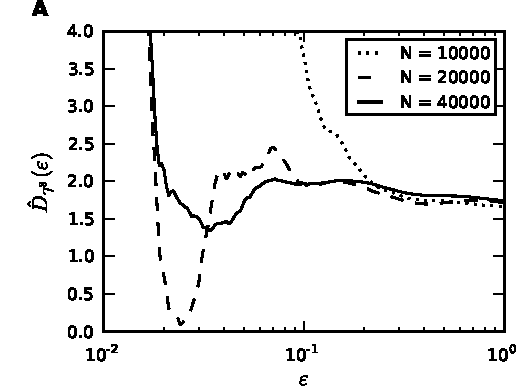
\includegraphics[width=.6\columnwidth]{transitivity3_dim_convergence.pdf} \\
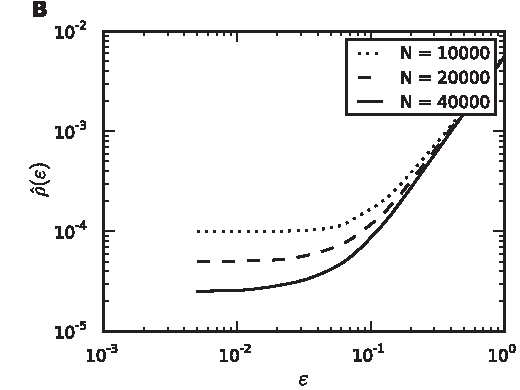
\includegraphics[width=.6\columnwidth]{recurrence_rates.pdf} \\
\caption{(A) Dependence of the transitivity dimension $\hat{D}_{\mathcal{T}}(\varepsilon)$ on the recurrence threshold $\varepsilon$ for realizations of the R\"ossler system (Eq.~\ref{eq:roessler}) with different lengths $N$ (sampling time $\Delta t=0.05$, first part of the trajectory removed to avoid possible transient dynamics). (B) Corresponding behavior of the edge density $\hat{\rho}$. Note the different scale on the $x$ axis.}
\label{fig:roessler_transitivity}
\end{figure}

Figure~\ref{fig:roessler_transitivity}A shows the behavior of the scale-dependent transitivity dimension estimate $\hat{D}_{\mathcal{T}}(\varepsilon)=\log(\hat{\mathcal{T}}(\varepsilon))/\log(3/4)$ for the R\"ossler system (Eq.~\ref{eq:roessler}) for three different RN sizes. We clearly recognize that $\hat{D}_{\mathcal{T}}(\varepsilon)$ assumes approximately stable (i.e., $N$- and $\varepsilon$-independent) values if the recurrence threshold is chosen sufficiently large. In general, there exist two limits that need to be taken into account: For too large recurrence rates, the RN characteristics lose their discriminatory skills, since too many edges are present masking subtle small-scale properties of the attractor~\cite{Donges2012PRE,Donner2010PRE}. In turn, if $\varepsilon$ is too low (e.g., if $\hat{\rho}$ is below the RN's percolation threshold)~\cite{Donges2012PRE}, the network decomposes into mutually disjoint components, and the resulting network characteristics can become ambiguous. In the considered example of the R\"ossler system, this decomposition is mainly caused by the rare excursions of some cycles towards larger $z$ values (cf.~Fig.~\ref{fig:attractor}), which give rise to a poorly populated region (low $p(x)$) of the attractor. In order to properly cover this part of the attractor for a given $\varepsilon$, many samples (i.e., a large network size $N$) are necessary. Otherwise, the edge density $\hat{\rho}$ starts saturating as $\varepsilon$ gets smaller (at least in the regime where most vertices close to the $z=0$ plane are still connected, cf. Fig.~\ref{fig:roessler_transitivity}B), and the transitivity dimension estimates strongly deviate from their expected values.

Notably, the analytical relationship (Eqs.~\ref{eq:dtu},\ref{eq:dtl}) between the effective (geometric) dimension of chaotic attractors and RN transitivity provides the theoretical justification and foundation for applying $\hat{\mathcal{T}}$ as a characteristic discriminating between high and low dynamical complexity of chaotic attractors. Unlike for $\hat{\mathcal{L}}$, the transitivity shows qualitatively the same behavior for discrete and time-continuous systems and is normalized, so that its values can be directly used as a quantitative measure of dynamical complexity associated with the effective geometric dimensionality and, hence, structural complexity of the attractor in phase space.

%{\color{red}Man sieht, dass $D_T(eps)$ erstmal konstant zu bleiben scheint bei etwas kleiner als 2 (konsistent mit Korrelationsdimension f??r R\"ossler immer etwas kleiner als 2). Wird die Schwelle eps zu klein, haben wir zu wenige Datenpunkte und die Sch\"atzung bricht zusammen. Entsprechend bricht die Sch\"atzung bei kleineren N schon bei gr????eren eps zusammen. Bei $N=40000$ haben wir das beste Ergebnis, wie zu erwarten war.}


\subsubsection{Other network characteristics}

In addition to the aforementioned characteristics, there are also other RN measures on both local and global scale that are able to trace changes in the dynamical complexity of a given system~\cite{Donges2011NPG,Zou2012aChaos,Zou2012bChaos}. In some cases, there are strong conceptual interrelationships with the previously discussed properties~\cite{Donges2011NPG}, whereas other measures (for example, the assortativity) require more complex considerations for providing potential interpretations of the observed variability. In general, we emphasize that as of today, transitivity and path length based characteristics provide the computationally simplest and theoretically best understood tracers of dynamical complexity based on RNs.


\subsubsection{Example: Tracing bifurcations in the R\"ossler system}
%\subsection{Detection of bifurcations}\label{sec:roessler_shrimp}

In order to illustrate the performance of RN transitivity $\hat{\mathcal{T}}$ and average path length $\hat{\mathcal{L}}$ as tracers for qualitative changes in the dynamics of complex systems, we briefly recall results originally obtained by the authors~\cite{Zou2010}. In the latter work, the RN properties have been successfully used to discriminate between periodic and chaotic solutions in a two-dimensional subspace ($a=b$) of the original three-dimensional parameter space of the R\"ossler system.

\begin{figure}
\centering
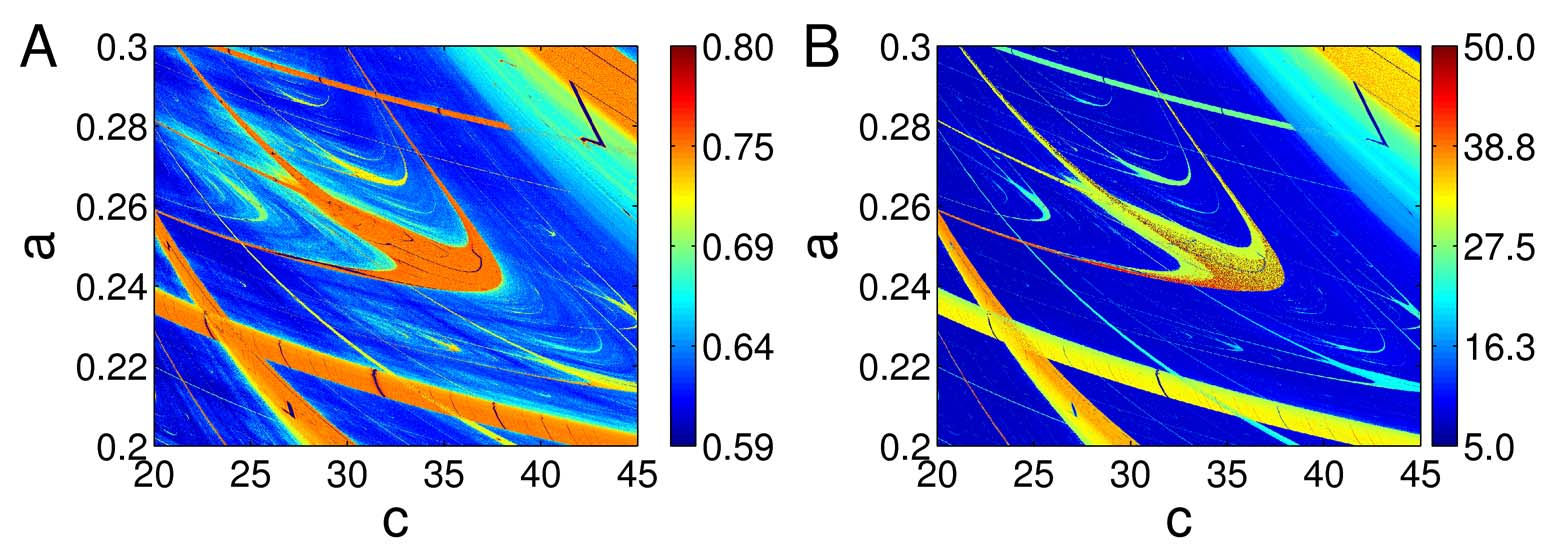
\includegraphics[width=\columnwidth]{ros_shrimp_eBook.pdf} 
\caption{RN transitivity $\hat{\mathcal{T}}$ (A) and average path length $\hat{\mathcal{L}}$ (B) for a two-dimensional intersection ($a=b$) of the three-dimensional parameter space of the R\"ossler system (Eq.~\ref{eq:roessler}), displaying ``shrimp'' structures (i.e., self-similar periodic windows with complex shape). For details, see~\cite{Zou2010}.}
\label{fig:roessler_shrimp}
\end{figure}

As Fig.~\ref{fig:roessler_shrimp} reveals, there are sequences of transitions between periodic and chaotic solutions. Specifically, we clearly see from the figure that the periodic windows are characterized by higher values of $\hat{\mathcal{T}}$ and $\hat{\mathcal{L}}$ than the chaotic solutions, which is in agreement with the general considerations discussed above. Specifically, for the periodic windows, we find $\hat{\mathcal{T}}$ close to $0.75$, the theoretical value for periodic dynamics (i.e., a system with effective dimension of $1$).

In a similar way, we may use the RN framework for capturing the signatures of qualitative changes in the attractor's shape and invariant density as a single control parameter is varied systematically. In a previous study using the R\"ossler system, we have investigated the RN properties across the transition from the classical phase-coherent R\"ossler attractor to the non-coherent funnel regime \cite{Zou2012aChaos}. Our results indicate that phase coherence -- in a similar spirit as fractal dimension -- should be characterized from a geometric rather than a dynamics viewpoint. However, as of today there is no single RN-based index for phase coherence that has been explicitly derived from theoretical considerations.

%\subsection{Dynamical transitions in transient dynamics}\label{sec:roessler_transient}

\begin{figure}
\centering
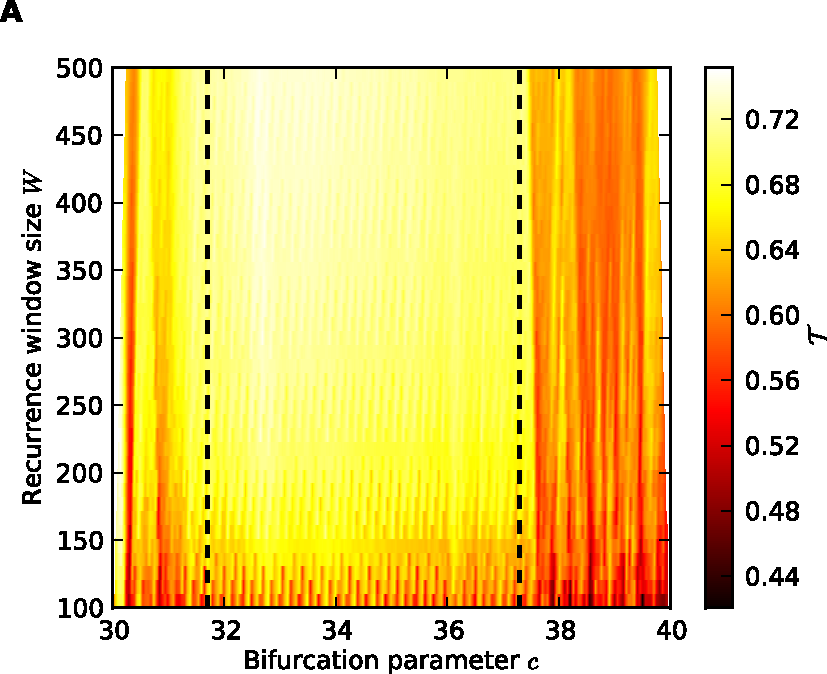
\includegraphics[width=0.485\columnwidth]{window_analysis_1_roessler_system.pdf} \hfill
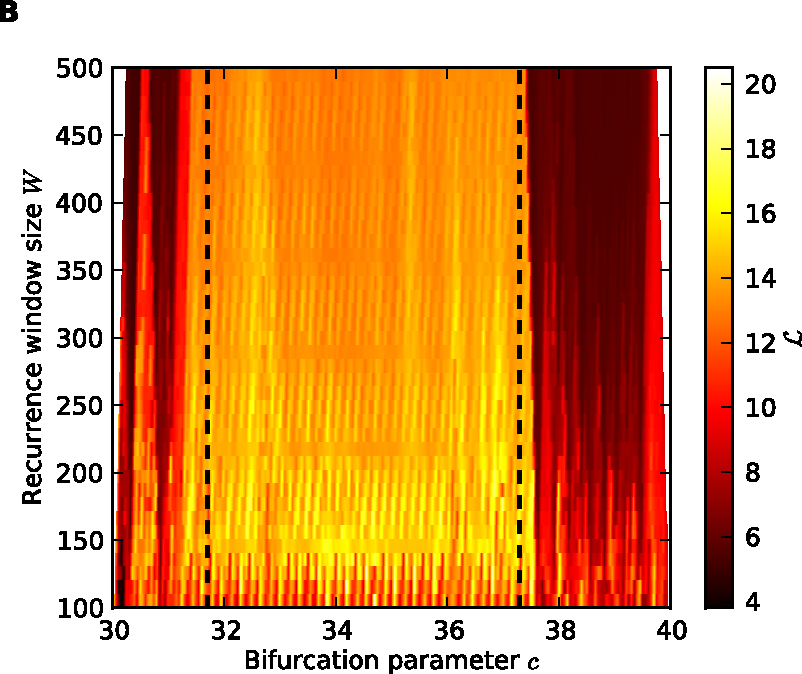
\includegraphics[width=0.485\columnwidth]{window_analysis_0_roessler_system.pdf} 
\caption{
(A) RN transitivity $\mathcal{T}$ and (B) average path length $\mathcal{L}$ for varying recurrence window size $W$ for the R\"ossler system (Eq.~\ref{eq:roessler}) at $a=b=0.25$ with linearly drifting bifurcation parameter $c$ over $10,000$ time steps (sampling interval $\Delta t=0.2$). For constructing the RN, a single long trajectory with the three original coordinates (i.e., no embedding) and initial values $(x_0,y_0,z_0)=(0,-10,0)$ was used. $W$ was varied linearly in the interval $(100,500)$, the recurrence window step size was fixed to $\Delta W=10$. The threshold $\varepsilon$ has been set such as to yield $\hat{\rho}=0.05$ in all windows. Vertical dashed lines indicate the critial values of $c$ marking transitions between periodic and chaotic windows at about $c=31.7$ and $37.3$, respectively (cf. Fig.~\ref{fig:roessler_shrimp}).}
\label{fig:roessler_transient}
\end{figure}

While the aforementioned results have been obtained for stationary systems, i.e., independent realizations of the system at fixed parameter values, tracing temporal changes in dynamical complexity of non-stationary systems is another interesting field of application with numerous examples in the real-world. Using model systems with drifting parameters such as the Lorenz \cite{Donges2011NPG} or R\"ossler systems (see Fig.~\ref{fig:roessler_transient}), it is possible to systematically evaluate the performance of RN characteristics in a sliding windows framework, underlining their capabilities for discriminating between qualitatively different types of dynamics and different degrees of complexity in non-stationary (transient) runs as well. For the example of a linearly drifting control parameter $c$ of the R\"ossler system (Fig.~\ref{fig:roessler_transient}), we find that the values at which bifurcations between periodic and chaotic behavior occur in the non-stationary system do well coincide with the numerically estimated bifurcation points of the autonomous system inferred from Fig.~\ref{fig:roessler_shrimp}, indicating that in the considered example, transient dynamics close to the bifurcation points does not play a major role as long as the considered RNs are still sufficiently large to obtain a reliable statistics.


\subsection{Characterization of local dimensionality}\label{sec:transitivity_local}

With the same rationale as for the global network transitivity, we can make use of the local clustering properties of RNs for defining local measures of attractor dimensionality, refered to as upper and lower clustering dimensions~\cite{Donner2011EPJB}:
\begin{eqnarray}
D_{\mathcal{C}}^u(x) &=& \limsup_{\varepsilon} \frac{\log(\mathcal{C}(x;\varepsilon))}{\log(3/4)}, \\
D_{\mathcal{C}}^l(x) &=& \liminf_{\varepsilon} \frac{\log(\mathcal{C}(x;\varepsilon))}{\log(3/4)}.
\end{eqnarray}
\noindent
Following the same argument as for the (global) transitivity dimensions, we do not need to consider the limit $\varepsilon\to 0$ here.

With similar considerations regarding the possible existence of two distinct accumulation points of $\mathcal{C}(x)$ as $\varepsilon$ varies, we may utilize this framework for characterizing the point-wise dimension of chaotic attractors in a unique way without making explicit use of scaling characteristics as in the common point-wise dimensions~\cite{Donner2011EPJB}. However, we need to keep in mind that the considered concept of (geometric) dimensionality is largely affected by the profile of the invariant density, e.g., the existence of sharp attractor boundaries or supertrack functions~\cite{Donner2010Nolta,Donner2011EPJB,Donner2010NJP}. For example, if the attractor has distinct tips (e.g., in the case of the H\'enon system~\cite{Donner2011EPJB,Donner2010NJP}), the geometric dimension at these points is effectively reduced to zero, which is reflected by $\hat{\mathcal{C}}_v=1$ for vertices $v$ sufficiently close to the tips. A similar behavior can be observed for the logistic map at the attractor boundaries and the supertrack functions~\cite{Donner2010Nolta,Donner2011EPJB,Donner2010NJP}.

The latter observations point to a prospective application of the local clustering properties of RNs. In case of chaotic attractors of time-continuous dynamical systems, it is known that an infinite number of unstable periodic orbits (UPOs) provide the skeleton of the chaotic dynamics and are densely embedded in the attractor. The localization of such UPOs is, however, known to be a challenging task. Since UPOs are relatively weakly repulsive (from a practical perspective, those UPOs with low periods are typically least unstable), a trajectory getting close to the vicinity of an UPO will stay close to this orbit for some finite amount of time~\cite{Lathrop1989}. As a result, the dynamics close to UPOs is quasi one-dimensional, and state vectors sampled from the trajectories approximate some lower-dimensional (in the limiting case one-dimensional) subset of the attractor manifold. In such case, the above theoretical considerations suggest that the local clustering coefficient $\hat{\mathcal{C}}_v$ of vertices $v$ close to low-periodic UPOs should be higher than the values typical for other parts of the chaotic attractor. This conceptual idea is supported by numerical results from our previous work~\cite{Donner2010PRE,Donner2010NJP} (cf.\, also the band structures with increased $\hat{\mathcal{C}}_v$ in Fig.~\ref{fig:local}B), but has not yet been systematically applied to the problem of UPO localization. Notably, the detection limit of UPOs should be ultimately determined by the recurrence threshold $\varepsilon$ in conjunction with the RN size $N$. Specifically, for every finite $\varepsilon>0$, there are infinitely many UPOs intersecting with the $\varepsilon$-neighborhood of some point $x_v$ in phase space, whereas we will (for a finite sample of state vectors) only resolve the signatures of the least unstable orbits.


\subsection{Cross-transitivity properties and coupling asymmetry}\label{sec:coupling}

The new class of statistical network measures designed for investigating the topology of networks of networks discussed in Section~\ref{sec:irn} is readily applicable for analyzing the interdependency structure of multiple complex dynamical systems. For the special case of two coupled systems $X$ and $Y$, we have demonstrated numerically that in an IRN, the asymmetry intrinsic to the global measures cross-transitivity $\hat{\mathcal{T}}^{XY}$ and global cross-clustering coefficient $\hat{\mathcal{C}}^{XY}$ can be exploited to reliably detect the direction of coupling between chaotic oscillators over a wide range of coupling strengths, requiring only a relatively small number of samples $N_{X,Y}\sim\mathcal{O}(10^2\dots 10^3)$~\cite{Feldhoff2012}. For this purpose, we make again use of the fact that transitivity-based characteristics quantify subtle geometric properties that can be easily evaluated both analytically and numerically. 

In order to see how cross-transitivities and global cross-clustering coefficients capture dynamical signatures of asymmetric vs. symmetric coupling configurations, let us assume a diffusive coupling with positive sign (i.e., an attractive interaction) as in Eq.~(\ref{eq:coupled_roessler}). In the uncoupled case, cross-triangles arise randomly according to the sampling from the systems' respective invariant densities. In this case, eventual asymmetries between $\hat{\mathcal{T}}^{XY}$ and $\hat{\mathcal{T}}^{YX}$ (or, equivalently, $\hat{\mathcal{C}}^{XY}$ and $\hat{\mathcal{C}}^{YX}$) originate from the geometry of the respective sets and the associated $p(x)$, which should already be reflected in the single-system RN transitivities and global clustering coefficients. In turn, if both systems are represented by the same set of state variables (a prerequisite for the application of IRNs) and obey similar values of $\hat{\mathcal{T}}^{X}$ and $\hat{\mathcal{T}}^{Y}$ ($\hat{\mathcal{C}}^{X}$ and $\hat{\mathcal{C}}^{Y}$), it is likely that also $\hat{\mathcal{T}}^{XY}$ and $\hat{\mathcal{T}}^{YX}$ ($\hat{\mathcal{C}}^{XY}$ and $\hat{\mathcal{C}}^{YX}$) take similar values. Note that minor asymmetries in the interdependent network characteristics can already occur if both systems are only weakly non-identical, e.g., when considering uncoupled identical R\"ossler systems with just a small detuning of their natural frequencies~\cite{Feldhoff2012}.

\begin{figure}[t!]
\centering
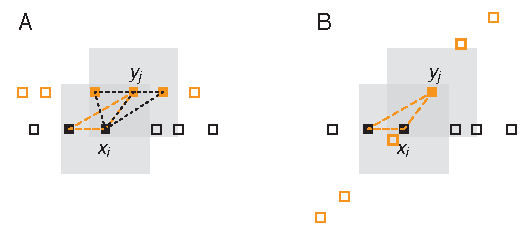
\includegraphics[width=\columnwidth]{clust_dimension.pdf}
\caption{Schematic illustration of the dimensionality and thus resulting mutual neighborhoods of state vectors $x_i$ and $y_j$ in the case of (A) uncoupled and (B) unidirectionally coupled systems. Shaded areas represent the neighborhoods of the respective state vectors, filled squares indicate recurrent states. In case (B), the coupling increases the driven system's dimension, so that formerly recurrent states are now outside of the neighborhood of $y_j$. Thus, the number of ``cross-triangles'' with baseline in $Y$ (i.e., ``from $X$ to $Y$'') decreases.}
\label{fig:clust_dimension}
\end{figure}

Let us suppose now that there is a unidirectional coupling $X\to Y$. In this case, the trajectory of the driven system $Y$ is attracted by that of the driver $X$ due to the considered form of coupling. As a result, it is likely to find more states in $Y$ that are close to mutually connected pairs of states in $X$ than in the uncoupled case. This implies that $\hat{\mathcal{T}}^{YX}$ ($\hat{\mathcal{C}}^{YX}$) increases since $X$ is ``pulling'' the trajectory of $Y$ and, hence, the number of triangles having their baseline in system $X$ increases relatively to those having their baseline in $Y$. Consequently, we expect to have $\hat{\mathcal{T}}^{YX}>\hat{\mathcal{T}}^{XY}$ and $\hat{\mathcal{C}}^{YX}>\hat{\mathcal{C}}^{XY}$, which is confirmed by numerical studies~\cite{Feldhoff2012}. An alternative way for understanding the observed asymmetry of the interdependent network characteristics is illustrated in Fig.~\ref{fig:clust_dimension}: moderate unidirectional coupling (below the onset of synchronization) increases the driven system's dimension \cite{Romano2007,zou2011} (we will numerically demonstrate this behavior in Section~\ref{sec:sync}), so that former neighbors of pairs of recurrent states in $X$ are not mutually close in $Y$ anymore. In this case, the number of ``cross-triangles'' with baseline in $Y$ decreases in comparison with those having their baseline in $X$. In fact, a corresponding decrease in $\hat{\mathcal{T}}^{XY}$ ($\hat{\mathcal{C}}^{XY}$) and an increase in $\hat{\mathcal{T}}^{YX}$ ($\hat{\mathcal{C}}^{YX}$) can often be observed in parallel (see Fig.~\ref{fig:roessler_coupling}).% (see Section~\ref{sec:roessler_coupling}).

%Inter-system recurrence network analysis is readily applicable to the analysis of paleoclimate data, since it does not require equidistant sampling or identical sampling times across multiple records (see above). A first successful application to detecting the predominant direction of coupling between the Indian and East Asian monsoon systems during the Holocene based on paleoclimate records of monsoonal variability from speleothems has been presented~\cite{Feldhoff2012}.

%\subsection{Detection of coupling asymmetry}\label{sec:roessler_coupling}

\begin{figure}
\centering
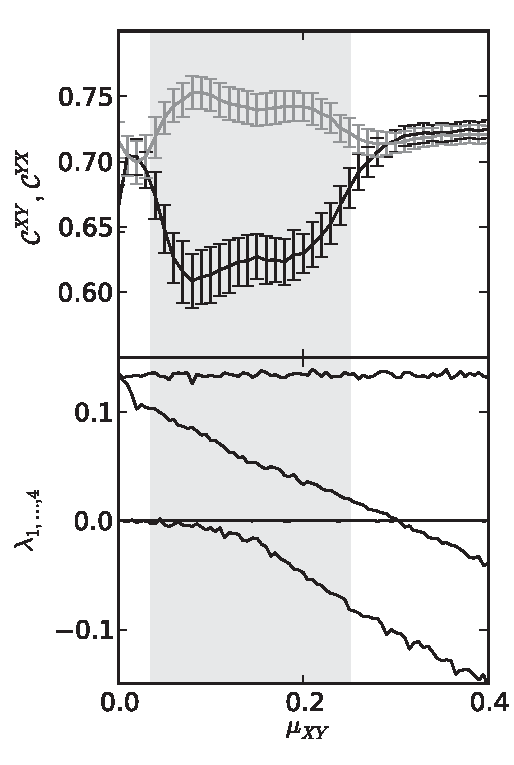
\includegraphics[width=.45\columnwidth]{FUN_XY.pdf} \hfill
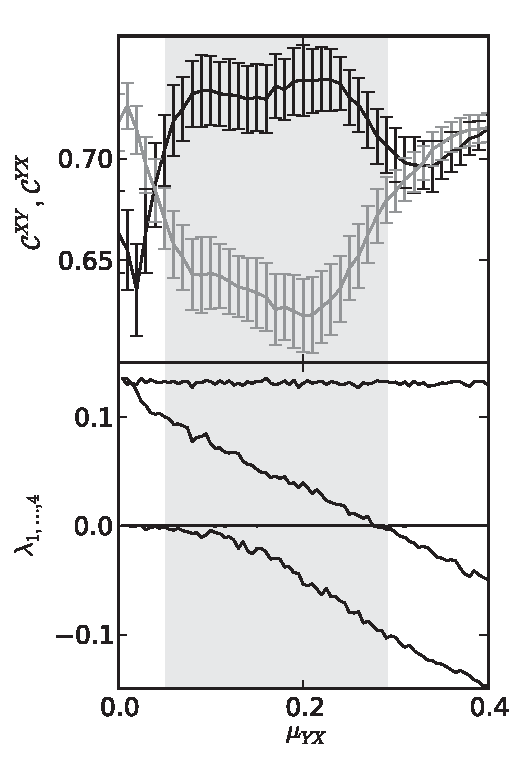
\includegraphics[width=.45\columnwidth]{FUN_YX.pdf} 
\caption{Global cross-clustering coefficients $\mathcal{C}^{XY}$ (black), $\mathcal{C}^{YX}$ (gray) and the four largest Lyapunov exponents $\lambda_{1,\dots,4}$ estimated using the Wolf algorithm~\cite{wolf1985} for two identically but slightly detuned ($\nu=0.02$) R\"ossler oscillators in the funnel regime subject to unidirectional coupling $X\to Y$ (left) and $Y\to X$ (right). The shaded regions mark the values of the coupling strength for which a correct identification of the coupling direction is achieved. Error bars represent mean values and standard deviations taken from an ensemble of 200 independent network realizations (with $N=1,500$ data points per system).}
\label{fig:roessler_coupling}
\end{figure}

Figure~\ref{fig:roessler_coupling} shows the illustrative example of global cross-clustering coefficients for two unidirectionally coupled R\"ossler systems in the funnel regime with the same parameters $a$, $b$ and $c$, but a weak detuning of $\nu=0.02$, following the setting of \cite{Feldhoff2012}. The obtained results are consistent with our above heuristic explanation for the emergence of asymmetries between the interdependent network characteristics in the presence of unidirectional coupling. Specifically, for a wide range of moderate coupling strengths, the difference between the two global cross-clustering coefficients allows to correctly identify the direction of the imposed coupling. At large coupling strengths (i.e., close to and beyond the onset of generalized synchronization, which is indicated by the second largest Lyapunov exponent of the system approaching zero as shown in Fig.~\ref{fig:roessler_coupling}), both global cross-clustering coefficients become statistically indistinguishable, which is consistent with the fact that the behavior of the driven system is completely locked to the dynamics of the driver (cf. Section~\ref{sec:sync}). In turn, the indistinguishability of both coupling directions at very low coupling strengths is most likely due to the fact that the geometric deformations of the driven system's attractor are too small to be detected by the given finite values of $\varepsilon_X$, $\varepsilon_Y$ and $\varepsilon_{XY}$ and the chosen network size. We expect that for larger IRNs and smaller distance thresholds, the lower boundary of the interval of coupling strengths for which the two global cross-clustering coefficients differ statistically significantly from each other will shift towards zero.

We emphasize that the same results can be obtained using the cross-transitivity replacing the global cross-clustering coefficient. Moreover, it is notable that the reported distinction can already be obtained at comparably small network sizes of some hundred vertices \cite{Feldhoff2012}.


\subsection{Joint transitivity properties and synchronization}\label{sec:sync}

The concept of joint recurrence plots (JRPs) has been found very useful for studying the otherwise hard to detect emergence of generalized synchronization (GS) between two coupled chaotic systems $X$ and $Y$~\cite{Romano2005EPL}. GS describes the presence of a general functional relationship between the trajectories of both systems, $y(t)=f(x(t))$, which can arise at sufficiently large coupling strengths in both uni- and bidirectional coupling configurations. Most available methods for identifying GS from time series data have been developed for driver-response relationships, and only few approaches are also suitable for studying GS in the presence of symmetric couplings~\cite{Feldhoff2013}. Among the latter, JRPs have recently attracted specific interest.

Romano~\textit{et~al.}~\cite{Romano2005EPL} argued that in case of GS, recurrences in the two coupled systems need to occur simultaneously (or with a given fixed time lag in the special case of lag synchronization, $y(t)=f(x(t-\tau))$). Hence, comparing the joint recurrence rate $JRR$ with the recurrence rates of the individual single-system RPs (taken to be the same for both systems) should show convergence of both values. The latter fact is quantified in terms of the \textit{joint probability of recurrence (JPR) index}
\begin{equation}
JPR = \max_{\tau} \frac{S(\tau)-RR}{1-RR}
\label{eq:jpr}
\end{equation}
\noindent
with the lagged joint recurrence rate ratio
\begin{equation}
S(\tau)=\frac{1}{N^2\, RR}\sum_{i,j=1}^N \Theta(\varepsilon_X-\|x_i-x_j\|)\, \Theta(\varepsilon_Y-\|y_{i+\tau}-y_{j+\tau}\|)
\end{equation}
\noindent
and $RR$ being the recurrence rate taken equal for both considered systems. Since for GS, we can expect that $S(\tau)\to 1$ for some $\tau$, $JPR\to 1$. However, the latter measure has some disadvantages. On the one hand, testing for significance of a specific value of $JPR$ usually requires complex surrogate data approaches for properly approximating the distribution of the underlying null hypothesis (no synchronization) adapted to the specific time series under study~\cite{Thiel2006}. On the other hand, comparing the single-system and joint recurrence rates may be insufficient since due to the complexity of fluctuations or the presence of stochastic components (observational noise), we hardly ever capture all single-system recurrence in the JRP. Consequently, a solely RR-based characterization does not necessarily lead to the expected ``optimum'' value of the synchronization index ($JPR=1$) in case of fully developed GS.

As an alternative, we have suggested that looking at higher-order characteristics (specifically, three-point instead of two-point relationships) may improve the results~\cite{Feldhoff2013}. %, especially when relying on probabilistic arguments. 
One convenient way is utilizing again the concept of transitivities from RN and JRN. The exploitation of alternative higher-order characteristics might be possible, but has not yet been explored.
%Joint recurrence networks can be analyzed by standard statistical measures from complex network theory~\cite{Newman2003,Donner2010b}, which, however, need to be reinterpreted in terms of the underlying systems' joint recurrence structure~\cite{Feldhoff2011,Feldhoff2012b,Donner2012c}. 
%Indeed, the transitivity properties of joint recurrence networks have been shown to reveal complex synchronization scenarios, notably including the detection of the onset of generalized synchronization, in coupled chaotic oscillators such as R\"ossler systems~\cite{Feldhoff2012b}. 
Notably, the specific requirements on the time series data render JRNs a promising approach for detecting intricate interconnections between qualitatively distinct observables in observational or experimental real-world data. 

As a heuristic indicator for the presence of GS, we have proposed using the \emph{transitivity ratio}~\cite{Feldhoff2013} 
\begin{equation}
\hat{Q}_{\mathcal{T}}=\frac{\hat{\mathcal{T}}^J}{(\hat{\mathcal{T}}^X+\hat{\mathcal{T}}^Y)/2}, 
\label{eq:qt}
\end{equation}
\noindent
i.e., the ratio between the JRN transitivity and the arithmic mean of the single-system RN transitivities. The rationale behind this definition is that for systems exhibiting GS, all degrees of freedom are completely locked, implying that both approach the same effective (fractal) dimension and should thus have the same RN transitivities, which approximately equal the JRN transitivity. Alternatively, we could also use other means of $\hat{\mathcal{T}}^{X,Y}$, such as the geometric or harmonic means, for obtaining a meaningful ratio. However, numerical experiments show that using the arithmetic mean provides values of $\hat{Q}_{\mathcal{T}}$ that are mostly confined to the interval $[0,1]$ with only minor exceedances in the fully developed GS regime~\cite{Feldhoff2013}. Since the arithmetic mean is always larger than the geometric one, normalizing with respect to the geometric mean $\sqrt{\hat{\mathcal{T}}^X\, \hat{\mathcal{T}}^Y}$ would lead to higher values of $\hat{Q}_{\mathcal{T}}$ and, hence, an even stronger violation of the desired normalization of the transitivity ratio. However, even when considering the normalization by the arithmetic mean of single-system RN transitivities, the thus defined transitivity ratio has two major drawbacks: 

On the one hand, if the single-system RN transitivities are essentially different (a case that has not been studied in~\cite{Feldhoff2013}), the contribution of the lower-dimensional system (higher transitivity) dominates the arithmetic mean in the denominator of Eq.~(\ref{eq:qt}) and, hence, the transitivity ratio itself irrespective of a possible well-defined driver-response relationship. 

On the other hand, there is no rigorous theoretical justification for $\hat{Q}_{\mathcal{T}}$ being a good indicator of GS. Notably, the definition of the transitivity ratio is based on the idea that the transitivities are related with the effective dimensions of the individual systems. In the uncoupled case, the degrees of freedom of both systems are independent; hence, the effective dimension of the composed system $X\otimes Y$ just reads $D^{X\otimes Y}=D^X + D^Y$ (notably, due to the logarithmic transform between RN transitivity and transitivity dimension, this additivity does \emph{not} apply to the RN transitivities). In turn, in case of GS, the degrees of freedom of both systems become mutually locked, leading to $D^{X\otimes Y}=D^X=D^Y$ (i.e., one system can be viewed as a -- possibly nonlinear -- projection of the other), with $D^X$ and $D^Y$ eventually differing from their values in the uncoupled case depending on the specific coupling configuration (e.g., uni- versus bidirectional coupling). 
%The latter fact is schematically depicted in Fig.~\ref{fig:dli}. 
Taking the estimated transitivity dimensions $\hat{D}_{\mathcal{T}^{X,Y}}$ as proxies for $D^{X,Y}$ and the \emph{pseudo-dimension} $\hat{\tilde{D}}_{\mathcal{T}^J}=\log(\hat{\mathcal{T}}^J)/\log(3/4)$ as an approximation of the true dimension $D^{X\otimes Y}$ of the composed system $X\otimes Y$\footnote{In fact, we should take here the transitivity dimension of the RN obtained for $X\otimes Y$, i.e., $\hat{D}_{\mathcal{T}^{X\otimes Y}}=\log(\hat{\mathcal{T}}^{X\otimes Y})/\log(3/4)$, which is in general not identical to the pseudo-dimension $\hat{\tilde{D}}_{\mathcal{T}^J}$ due to the different metrics used for the definition of recurrences of $X\otimes Y$ and joint recurrences of $X$ and $Y$.}, the latter case would translate into $\hat{Q}_{\mathcal{T}}=1$, which is approximately attained in numerical studies for coupled R\"ossler systems in different dynamical regimes~\cite{Feldhoff2013}.

%\begin{figure}
%\centering
%\includegraphics[width=\columnwidth]{JRN_nosync_sync.pdf} 
%\caption{Schematic representation of the degrees of freedom determining the properties of RN and JRN: (A) Uncoupled case: the degrees of freedom of $X$ and $Y$ are independent, visualized by pairwise orthogonal unit vectors $e_i^{X,Y}$ spanning the phase spaces of $X$ and $Y$. (B) Generalized synchronization: the degrees of freedom of both systems are fully locked, visualized by pairwise parallel unit vectors.}
%\label{fig:dli}
%\end{figure}

In order to circumvent both problems, we suggest here utilizing an alternative indicator, which is directly based on the concept of effective dimensions (degrees of freedom) of the individual systems. In analogy with the mutual information (sometimes also called redundancy \cite{Palus1995,Prichard1995}) frequently used in nonlinear time series analysis, we define the \emph{transitivity dimension redundancies}
\begin{eqnarray}
\hat{\tilde{D}}_{\mathcal{T}^R}&=&\hat{D}_{\mathcal{T}^X}+\hat{D}_{\mathcal{T}^Y}-\hat{\tilde{D}}_{\mathcal{T}^J}, \\
\hat{D}_{\mathcal{T}^R}&=&\hat{D}_{\mathcal{T}^X}+\hat{D}_{\mathcal{T}^Y}-\hat{D}_{\mathcal{T}^{X\otimes Y}},
\end{eqnarray}
\noindent
which should assume zero values in the uncoupled case and exhibit $\hat{D}_{\mathcal{T}^X}=\hat{D}_{\mathcal{T}^Y}=\hat{D}_{\mathcal{T}^{X\otimes Y}}=\hat{\tilde{D}}_{\mathcal{T}^J}$ in case of GS. In order to obtain a normalized measure for the presence of GS, we define the \emph{dimensional locking index (DLI)}
\begin{eqnarray}
\widehat{\widetilde{DLI}} &=& \frac{\hat{\tilde{D}}_{\mathcal{T}^R}}{\hat{\tilde{D}}_{\mathcal{T}^J}}, \\
\widehat{DLI} &=& \frac{\hat{D}_{\mathcal{T}^R}}{\hat{D}_{\mathcal{T}^{X\otimes Y}}}.
\end{eqnarray}
\noindent
Notably, this index is tailored to the dimensionality interpretation of RN transitivity. In a strict sense, this argument only applies if using the single-system RN transitivity (dimension) of the composed system $X\otimes Y$ instead of the JRN transitivity (dimension) $\hat{\tilde{D}}_{\mathcal{T}^J}$. However, at this point, we suggest using the latter as an approximation. A detailed comparison between the two definitions will be subject to future research.

\begin{figure}
\centering
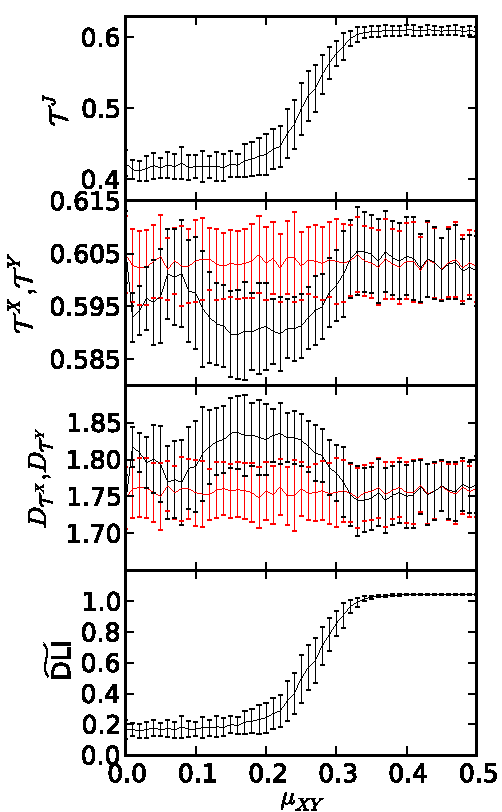
\includegraphics[width=.45\columnwidth]{funnelK51R100+nu.pdf} \hfill
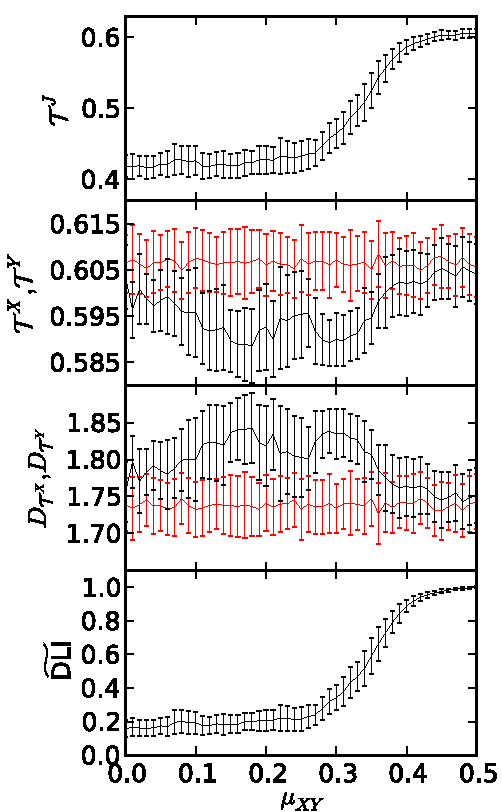
\includegraphics[width=.45\columnwidth]{funnelK51R100-nu.pdf} 
\caption{Joint transitivity $\hat{\mathcal{T}}_J$, single-system RN transitivities $\hat{\mathcal{T}}_{X,Y}$, corresponding transitivity dimensions $\hat{D}_{\mathcal{T}_X}$, $\hat{D}_{\mathcal{T}_Y}$ and derived dimensional locking index $\widehat{\widetilde{DLI}}$ (from top to bottom) for two unidirectionally coupled R\"ossler systems ($X\to Y$) in the funnel regime with $\nu=0.02$ (driver oscillates faster than driven system, left panels) and $\nu=-0.02$ (right panels). The error bars indicate mean values and standard deviations estimated from 100 independent network realizations for each value of the coupling strength $\mu_{XY}$. For transitivities and transitivity dimensions, red (black) lines correspond to the values for system $X$ ($Y$).}
\label{fig:roessler_sync}
\end{figure}

In order to further illustrate the behavior of the (J)RN-based characteristics for detecting the emergence of GS, we reconsider the example of two unidirectionally coupled identical but slightly detuned R\"ossler systems from Section~\ref{sec:coupling}. In contrast to \cite{Feldhoff2013}, who studied different settings for uni- and bidirectional configurations with single realizations of the same system, we present here results obtained from ensembles of realizations. The results shown in Fig.~\ref{fig:roessler_sync} demonstrate that the estimated values of $\mathcal{T}^J$ and $\widetilde{DLI}$ exhibit a marked increase at the onset of GS. Specifically, the new $DLI$ index approaches one (with little overshooting) in the synchronized regime as expected, but takes values of only about $0.2$ or lower in the non-synchronous case (in comparison with values of about $0.7$ exhibited by $Q_{\mathcal{T}}$, cf. Fig.~2B in \cite{Feldhoff2013}). 

As a second important observation, we find a systematic and significant decrease in the RN transitivity of the driven system at moderate coupling strengths before the onset of GS, which corresponds to an increase of the associated transitivity dimension. This behavior is precisely what was claimed in the context of coupling analysis in Section~\ref{sec:coupling} for providing an explanation of the numerically observed asymmetry between the transitivity-based interdependent network characteristics. These results underline that some integrated utilization of single-system, inter-system and joint recurrence networks can eventually provide deep insights into the coupling regime and strength from bivariate observations.


\subsection{Real-world applications}

Although much recent work on RNs and multivariate generalizations thereof has been focused on the development of the theoretical framework and its numerical exploration using simple low-dimensional model systems, there have already been some first successful applications to characterizing system's properties from experimental or observational time series.


\subsubsection{Applications in climatology}

One important field of recent applications is paleoclimatology, which has already been taken as an illustrative example in the seminal paper by Marwan \textit{et~al.} \cite{Marwan2009}. The corresponding study was later extended to some systematic investigation of the temporal variability profile of RN-based complexity measures for three marine sediment records of terrigenous dust flux off Africa during the last 5 million years. Donges \textit{et~al.} \cite{Donges2011NPG} argued that RNs can be used for characterizing dynamics from non-uniformly sampled or age-uncertain data, since this methodological approach does not make explicit use of time information. In turn, due to the necessity of using time-delay embedding, there is implicit time information entering the analysis, which has been recognized but widely neglected in previous works. Notably, disregarding age uncertainty and sampling heterogeneity appears a reasonable approximation only in cases where the distribution of instantaneous sampling rates remains acceptably narrow. 

The results of Donges \textit{et~al.} \cite{Donges2011PNAS} pointed to the existence of spatially coherent changes in the long-term variability of environmental conditions over Africa, which have probably influenced the evolution of human ancestor species. Specifically, RN transitivity and average path length have been interpreted as indicators for ``climate regularity'' (i.e., the complexity of fluctuations as captured by the transitivity dimensions) and ``abrupt dynamical changes'', respectively. By identifying three time intervals with consistent changes of the RN properties obtained from spatially widely separated records, it has been possible to attribute the corresponding long-term changes in the dynamics to periods characterized by known or speculated mechanisms for large-scale climate shifts such as changes in the Indian ocean circulation patterns, the intensification of the atmospheric Walker circulation, or changes in the dominant periodicity of Northern hemispheric glacial cycles. Moreover, Donges \textit{et~al.} \cite{Donges2011NPG} demonstrated a good robustness of the results of RN analysis obtained in a sliding windows framework when varying the corresponding parameters (e.g., window size or embedding delay) over a reasonable range.

As another methodological step towards better understanding climatic mechanisms, we have used two speleothem records for studying interdependencies between the two main branches of the Asian summer monsoon (the Indian and East Asian summer monsoon) by means of IRNs~\cite{Feldhoff2012}. For this purpose, they selected two data sets of oxygen isotope anomalies from speleothems obtained from two caves in China and the Oman, respectively, which can be considered as proxies for the annual precipitation and, hence, the overall strength of the two monsoon branches over the last about 10,000 years. The asymmetries of the IRN cross-transitivities and global cross-clustering coefficients provided clear evidence for a marked influence of the Indian summer monsoon on the East Asian branch rather than vice versa, which is in good agreement with existing climatological theories. As a subsequent extension of this work, we emphasize the possibility of repeating the same kind of analysis in a sliding windows framework, thereby gaining information on possible temporal changes of the associated climatic patterns during certain time periods as recently revealed using correlation-based complex network analysis applied to a larger set of speleothem records from the Asian monsoon domain \cite{Rehfeld2012}.

In order to characterize dynamical complexity associated with more recent environmental variability, Lange and B\"ose \cite{Boese2012,Lange2013Book} used RQA as well as RN analysis for studying global photosynthetic activity from remote sensing data in conjunction with global precipitation patterns. Specifically, they studied 14-years long time series (1998-2011) of the fraction of absorbed photosynthetically active radiation (faPAR) with a spatial resolution of 0.5$^o$ around the Earth and a temporal sampling of about ten days, providing time series of $N=504$ data points. Their results revealed very interesting spatial complexity patterns, which have been largely, but not exclusively determined by the amplitude of the annual cycle of vegetation growth in different ecosystems.


\subsubsection{Applications in fluid dynamics}

In a series of papers, Gao \textit{et~al.} investigated the emerging complexity of dynamical patterns in two-phase gas-liquid or oil-water flows in different configurations using RN techniques. In general, multiple sensors measuring fluctuations of electrical conductance have been used for obtaining signals that are characteristic for the different flow patterns. For gas-liquid two-phase upward flows in vertical pipes, different types of complex networks generated from observational data have been proposed, among which the degree correlations (assortativity) of RNs was proven to be particularly useful for distinguishing between qualitatively different flow types \cite{Gao2009}. For oil-water two-phase upward flows in a similar configuration, the global clustering coefficient of RNs reveals a marked increase in dynamical complexity (detectable in terms of a decreasing $\hat{\mathcal{C}}$) as the flow pattern changes from slug flow over coarse to very finely dispersed bubble flow \cite{Gao2013PLA}. In case of oil-water two-phase flows in inclined pipes \cite{Gao2010PRE}, the motif distributions of RNs (specifically, the frequency distributions of small subgraphs containing exactly four vertices) revealed an increasing degree of heterogeneity, where the motif ranking was conserved in all experimental conditions, whereas the absolute motif frequency dramatically changed. The corresponding results were independently confirmed using some classical measures of complexity, which indicated increasing complexity in conjunction with increasing heterogeneity of the RN motif distributions. Finally, for characterizing horizontal oil-water flows \cite{Gao2013EPL}, RN and IRN analysis were combined for studying conductance signals from multiple sensors. Specifically, cross-transitivity was found a useful measure for tracing the transitions between stable stratified and unstable states associated with the formation of droplets.


\subsubsection{Applications in electrochemistry}

Zou \textit{et~al.} \cite{Zou2012bChaos} studied the complexity of experimental electrochemical oscillations as one control parameter of the experiments (temperature) was systematically varied. By utilizing a multitude of complementary RN characteristics, they could demonstrate a systematic rise in dynamical complexity as temperature increased, but an absence of a previously speculated phase transition \cite{wickramasinghe_chaos_2010} separating phase-coherent from noncoherent chaotic oscillations. The latter results were independently confirmed using other classical indicators for phase coherence, as well as studies of a corresponding mathematical model of the specific electrochemical processes.


\subsubsection{Applications in medicine}

Finally, there have been a couple of successful applications in a medical context. Marwan \textit{et~al.} \cite{Marwan2010Biosignal} demonstrated that the global clustering coefficients of RNs obtained from heartbeat intervals, diastolic and systolic blood pressure allowed a reliable identification of patients with pre-eclampsia, a cardiovascular disease during pregnancy with a high risk of fetal and maternal morbidity. Their results were further improved by Ram\'{i}rez \textit{et~al.} \cite{Ramirez2012,Ramirez2013} who considered combinations of various RN-based network characteristics. In a similar spirit as for cardiovascular diseases, recent results point to the capability of RN characteristics for discriminating between the EEG signals of healthy and epileptic patients \cite{Subramaniyam2013}.


\section{Related approaches}

Besides the recurrence definition based on a fixed distance threshold $\varepsilon$ in phase space (i.e., equal neighborhood volumes around all available state vectors), there are alternative ways for defining recurrences and, hence, RPs and RNs. For example, the original definition of a RP by Eckmann \textit{et~al.} \cite{Eckmann1987} makes use of $k$-nearest neighbors (i.e., a fixed probability mass of the considered neighborhoods). Re-interpreting the resulting recurrence matrix as the adjacency matrix of a complex network leads to a different type of RN \cite{Shimada2008}, typically refered to as \emph{$k$-nearest neighbor network}. Since in this definition, the neighborhood relation is not symmetric (i.e., $x_j$ being among the $k$ nearest neighbors of $x_i$ does not imply $x_i$ also being among the $k$ nearest neighbors of $x_j$), the resulting networks are in general directed graphs, and the local density of unidirectional edges (as opposed to bidirectional ones) is related to the gradient of the invariant density.

In order to circumvent the directedness of $k$-nearest neighbor networks, Xu \textit{et~al.} \cite{Small2009,Xu2008} proposed an algorithm for balancing the neighborhood relationships in such a way that they become symmetric again. The resulting networks embedded in phase space, sometimes also refered to as \emph{adaptive nearest neighbor networks} \cite{Donner2011IJBC}, are conceptually more similar to classical ($\varepsilon$-)RNs, but still exhibit somewhat different topological characteristics. In particular, the motif distribution of adaptive nearest neighbor networks has been shown to allow a discrimination between different types of dynamics in terms of a different motif ranking \cite{Liu2010,Xu2008}. Consequently, this approach has been mainly used for such discriminatory tasks, including applications to turbulence phenomena, stock markets \cite{Liu2010} or instrumental music \cite{Donner2011IJBC}.

For a detailed discussion of the differences between $\varepsilon$-RNs, $k$-nearest neighbor and adaptive nearest neighbor networks, we refer to \cite{Donner2011IJBC}. While these three classes of time series networks exhibit very strong conceptual similarities (the same applies to correlation networks \cite{Yang2008} if interpreting the correlation coefficient between two sufficiently high-dimensional state vectors as a generalized distance), the approach proposed by Li \textit{et~al.} \cite{Li2011a,Li2011b} can be understood as being derived from the RN idea. Here, for a set of $m$-dimensional embedding vectors, all mutual Euclidean distances are computed. Based on the maximum point-wise Euclidean distance $d_{max}(m)$, the threshold distance of an RN is taken as $\varepsilon(m)=d_{max}(m)/(N-1)$. This procedure is repeated for different $m$, and the critical value of the embedding dimension for which the resulting network gets completely disconnected is interpreted as a complexity index \cite{Cao2013}. However, it has not yet been demonstrated that this algorithmic approach has any conceptual benefits in comparison with the classical RN transitivity obtained for a fixed embedding dimension.

Another conceptual approach loosely related to RNs provides the foundation of the frequency-degree mapping algorithm introduced by Li \textit{et~al.} \cite{Li2012}. Here, the resulting time series networks contain two types of edges: (i) temporal edges connecting subsequent points in time, and (ii) proximity edges containing observations of similar values, where similarity is defined by an initial grouping of the data into a discrete set of classes, and observed values being connected if and only if they belong to the same class. Notably, the latter approach combines the classical recurrence idea and basic concepts of symbolic dynamics \cite{Daw2003}. In this spirit, the resulting network's adjacency matrix is given as the recurrence matrix associated with a symbolic recurrence plot \cite{Donner2008,Faure2010,Graben2013} plus a ``stripe'' around the matrix' main diagonal. The frequency-degree mapping algorithm has been successfully applied to characterizing signatures of various types of ventricular arrhytmias in human heart beat time series \cite{Li2012}.

%
%{\color{red}
%visibility graph similarity,...
%
%transformation from networks to time series (Shimada)
%}


\section{Summary}

This work has provided an overview on the current state of complex network approaches to quantifying nonlinear dynamics based on recurrence plots. This emerging field has already proven its great potentials by addressing methodological questions common to various fields of research, such as the characterization of complexity, the identification of dynamical transitions in non-stationary time series, and the detection of asymmetric coupling and generalized synchronization from bivariate records. In all these areas, recurrence networks and multivariate generalizations thereof have been successfully applied to model systems and at least partially also to real-world observational or experimental data. The results available so far suggest reasonable numerical properties and, hence, a wide applicability of this approach. Moreover, the quantitative analysis of recurrence networks is supported by a rigorous analytical framework derived from the theory of random geometric graphs. In turn, unlike other recurrence plot-based analysis concepts, recurrence networks characterize geometric properties of the system under study rather than dynamical ones. However, since geometry and dynamics are known to be closely interrelated, the network-based approach is still useful for obtaining information on dynamical complexity and related aspects as reflected in the system's structural features.

Beyond exclusively reviewing recent results, we have also discussed some new aspects not yet found in the previous peer-reviewed literature: (i) an analytical framework for inter-system recurrence networks providing a possible foundation for a future analytical understanding of geometric signatures of coupling between dynamical systems, (ii) a straightforward extension of joint recurrence plots and joint recurrence networks to a less restrictive definition, which could allow studying synchronization processes between noisy systems based on recurrence plots, and (iii) the introduction of a new index for generalized synchronization, which is expected to yield a better performance than other recent recurrence-based indices. The latter three aspects open new perspectives for both an improved theoretical understanding of geometric effects of coupling and synchronization and applications in various contexts. We outline corresponding further investigations as an important research avenue for our future work.


%\section{Future perspectives???}


%\section{Section Heading}
%\label{sec:1}
%Use the template \emph{chapter.tex} together with the Springer document class SVMono (monograph-type books) or SVMult (edited books) to style the various elements of your chapter content in the Springer layout.
%
%Instead of simply listing headings of different levels we recommend to
%let every heading be followed by at least a short passage of text.
%Further on please use the \LaTeX\ automatism for all your
%cross-references and citations. And please note that the first line of
%text that follows a heading is not indented, whereas the first lines of
%all subsequent paragraphs are.
%
%\section{Section Heading}
%\label{sec:2}
%% Always give a unique label
%% and use \ref{<label>} for cross-references
%% and \cite{<label>} for bibliographic references
%% use \sectionmark{}
%% to alter or adjust the section heading in the running head
%Instead of simply listing headings of different levels we recommend to
%let every heading be followed by at least a short passage of text.
%Further on please use the \LaTeX\ automatism for all your
%cross-references and citations.
%
%Please note that the first line of text that follows a heading is not indented, whereas the first lines of all subsequent paragraphs are.
%
%Use the standard \verb|equation| environment to typeset your equations, e.g.
%%
%\begin{equation}
%a \times b = c\;,
%\end{equation}
%%
%however, for multiline equations we recommend to use the \verb|eqnarray| environment\footnote{In physics texts please activate the class option \texttt{vecphys} to depict your vectors in \textbf{\itshape boldface-italic} type - as is customary for a wide range of physical subjects}.
%\begin{eqnarray}
%a \times b = c \nonumber\\
%\vec{a} \cdot \vec{b}=\vec{c}
%\label{eq:01}
%\end{eqnarray}
%
%\subsection{Subsection Heading}
%\label{subsec:2}
%Instead of simply listing headings of different levels we recommend to
%let every heading be followed by at least a short passage of text.
%Further on please use the \LaTeX\ automatism for all your
%cross-references\index{cross-references} and citations\index{citations}
%as has already been described in Sect.~\ref{sec:2}.
%
%\begin{quotation}
%Please do not use quotation marks when quoting texts! Simply use the \verb|quotation| environment -- it will automatically render Springer's preferred layout.
%\end{quotation}
%
%
%\subsubsection{Subsubsection Heading}
%Instead of simply listing headings of different levels we recommend to
%let every heading be followed by at least a short passage of text.
%Further on please use the \LaTeX\ automatism for all your
%cross-references and citations as has already been described in
%Sect.~\ref{subsec:2}, see also Fig.~\ref{fig:1}\footnote{If you copy
%text passages, figures, or tables from other works, you must obtain
%\textit{permission} from the copyright holder (usually the original
%publisher). Please enclose the signed permission with the manucript. The
%sources\index{permission to print} must be acknowledged either in the
%captions, as footnotes or in a separate section of the book.}
%
%Please note that the first line of text that follows a heading is not indented, whereas the first lines of all subsequent paragraphs are.
%
%% For figures use
%%
%\begin{figure}[b]
%\sidecaption
%% Use the relevant command for your figure-insertion program
%% to insert the figure file.
%% For example, with the graphicx style use
%%\includegraphics[scale=.65]{figure}
%%
%% If no graphics program available, insert a blank space i.e. use
%%\picplace{5cm}{2cm} % Give the correct figure height and width in cm
%%
%\caption{If the width of the figure is less than 7.8 cm use the \texttt{sidecapion} command to flush the caption on the left side of the page. If the figure is positioned at the top of the page, align the sidecaption with the top of the figure -- to achieve this you simply need to use the optional argument \texttt{[t]} with the \texttt{sidecaption} command}
%\label{fig:1}       % Give a unique label
%\end{figure}
%
%
%\paragraph{Paragraph Heading} %
%Instead of simply listing headings of different levels we recommend to
%let every heading be followed by at least a short passage of text.
%Further on please use the \LaTeX\ automatism for all your
%cross-references and citations as has already been described in
%Sect.~\ref{sec:2}.
%
%Please note that the first line of text that follows a heading is not indented, whereas the first lines of all subsequent paragraphs are.
%
%For typesetting numbered lists we recommend to use the \verb|enumerate| environment -- it will automatically render Springer's preferred layout.
%
%\begin{enumerate}
%\item{Livelihood and survival mobility are oftentimes coutcomes of uneven socioeconomic development.}
%\begin{enumerate}
%\item{Livelihood and survival mobility are oftentimes coutcomes of uneven socioeconomic development.}
%\item{Livelihood and survival mobility are oftentimes coutcomes of uneven socioeconomic development.}
%\end{enumerate}
%\item{Livelihood and survival mobility are oftentimes coutcomes of uneven socioeconomic development.}
%\end{enumerate}
%
%
%\subparagraph{Subparagraph Heading} In order to avoid simply listing headings of different levels we recommend to let every heading be followed by at least a short passage of text. Use the \LaTeX\ automatism for all your cross-references and citations as has already been described in Sect.~\ref{sec:2}, see also Fig.~\ref{fig:2}.
%
%For unnumbered list we recommend to use the \verb|itemize| environment -- it will automatically render Springer's preferred layout.
%
%\begin{itemize}
%\item{Livelihood and survival mobility are oftentimes coutcomes of uneven socioeconomic development, cf. Table~\ref{tab:1}.}
%\begin{itemize}
%\item{Livelihood and survival mobility are oftentimes coutcomes of uneven socioeconomic development.}
%\item{Livelihood and survival mobility are oftentimes coutcomes of uneven socioeconomic development.}
%\end{itemize}
%\item{Livelihood and survival mobility are oftentimes coutcomes of uneven socioeconomic development.}
%\end{itemize}
%
%\begin{figure}[t]
%\sidecaption[t]
%% Use the relevant command for your figure-insertion program
%% to insert the figure file.
%% For example, with the option graphics use
%%\includegraphics[scale=.65]{figure}
%%
%% If no graphics program available, insert a blank space i.e. use
%%\picplace{5cm}{2cm} % Give the correct figure height and width in cm
%%
%%\caption{Please write your figure caption here}
%\caption{If the width of the figure is less than 7.8 cm use the \texttt{sidecapion} command to flush the caption on the left side of the page. If the figure is positioned at the top of the page, align the sidecaption with the top of the figure -- to achieve this you simply need to use the optional argument \texttt{[t]} with the \texttt{sidecaption} command}
%\label{fig:2}       % Give a unique label
%\end{figure}
%
%\runinhead{Run-in Heading Boldface Version} Use the \LaTeX\ automatism for all your cross-references and citations as has already been described in Sect.~\ref{sec:2}.
%
%\subruninhead{Run-in Heading Italic Version} Use the \LaTeX\ automatism for all your cross-refer\-ences and citations as has already been described in Sect.~\ref{sec:2}\index{paragraph}.
%% Use the \index{} command to code your index words
%%
%% For tables use
%%
%\begin{table}
%\caption{Please write your table caption here}
%\label{tab:1}       % Give a unique label
%%
%% Follow this input for your own table layout
%%
%\begin{tabular}{p{2cm}p{2.4cm}p{2cm}p{4.9cm}}
%\hline\noalign{\smallskip}
%Classes & Subclass & Length & Action Mechanism  \\
%\noalign{\smallskip}\svhline\noalign{\smallskip}
%Translation & mRNA$^a$  & 22 (19--25) & Translation repression, mRNA cleavage\\
%Translation & mRNA cleavage & 21 & mRNA cleavage\\
%Translation & mRNA  & 21--22 & mRNA cleavage\\
%Translation & mRNA  & 24--26 & Histone and DNA Modification\\
%\noalign{\smallskip}\hline\noalign{\smallskip}
%\end{tabular}
%$^a$ Table foot note (with superscript)
%\end{table}
%%
%\section{Section Heading}
%\label{sec:3}
%% Always give a unique label
%% and use \ref{<label>} for cross-references
%% and \cite{<label>} for bibliographic references
%% use \sectionmark{}
%% to alter or adjust the section heading in the running head
%Instead of simply listing headings of different levels we recommend to
%let every heading be followed by at least a short passage of text.
%Further on please use the \LaTeX\ automatism for all your
%cross-references and citations as has already been described in
%Sect.~\ref{sec:2}.
%
%Please note that the first line of text that follows a heading is not indented, whereas the first lines of all subsequent paragraphs are.
%
%If you want to list definitions or the like we recommend to use the Springer-enhanced \verb|description| environment -- it will automatically render Springer's preferred layout.
%
%\begin{description}[Type 1]
%\item[Type 1]{That addresses central themes pertainng to migration, health, and disease. In Sect.~\ref{sec:1}, Wilson discusses the role of human migration in infectious disease distributions and patterns.}
%\item[Type 2]{That addresses central themes pertainng to migration, health, and disease. In Sect.~\ref{subsec:2}, Wilson discusses the role of human migration in infectious disease distributions and patterns.}
%\end{description}
%
%\subsection{Subsection Heading} %
%In order to avoid simply listing headings of different levels we recommend to let every heading be followed by at least a short passage of text. Use the \LaTeX\ automatism for all your cross-references and citations citations as has already been described in Sect.~\ref{sec:2}.
%
%Please note that the first line of text that follows a heading is not indented, whereas the first lines of all subsequent paragraphs are.
%
%\begin{svgraybox}
%If you want to emphasize complete paragraphs of texts we recommend to use the newly defined Springer class option \verb|graybox| and the newly defined environment \verb|svgraybox|. This will produce a 15 percent screened box 'behind' your text.
%
%If you want to emphasize complete paragraphs of texts we recommend to use the newly defined Springer class option and environment \verb|svgraybox|. This will produce a 15 percent screened box 'behind' your text.
%\end{svgraybox}
%
%
%\subsubsection{Subsubsection Heading}
%Instead of simply listing headings of different levels we recommend to
%let every heading be followed by at least a short passage of text.
%Further on please use the \LaTeX\ automatism for all your
%cross-references and citations as has already been described in
%Sect.~\ref{sec:2}.
%
%Please note that the first line of text that follows a heading is not indented, whereas the first lines of all subsequent paragraphs are.
%
%\begin{theorem}
%Theorem text goes here.
%\end{theorem}
%%
%% or
%%
%\begin{definition}
%Definition text goes here.
%\end{definition}
%
%\begin{proof}
%%\smartqed
%Proof text goes here.
%\qed
%\end{proof}
%
%\paragraph{Paragraph Heading} %
%Instead of simply listing headings of different levels we recommend to
%let every heading be followed by at least a short passage of text.
%Further on please use the \LaTeX\ automatism for all your
%cross-references and citations as has already been described in
%Sect.~\ref{sec:2}.
%
%Note that the first line of text that follows a heading is not indented, whereas the first lines of all subsequent paragraphs are.
%%
%% For built-in environments use
%%
%\begin{theorem}
%Theorem text goes here.
%\end{theorem}
%%
%\begin{definition}
%Definition text goes here.
%\end{definition}
%%
%\begin{proof}
%\smartqed
%Proof text goes here.
%\qed
%\end{proof}
%

\begin{acknowledgement}
The reported development of the recurrence network framework has been a community effort. Among other colleagues, we particularly acknowledge important contributions by Jobst Heitzig and Norbert Marwan, as well as multiple inspiring discussions with J\"urgen Kurths. Financial support of this work has been granted by the German Federal Environmental Agency, the European Union Seventh Framework Program, the Max Planck Society, the Stordalen Foundation, the German Research Association via the IRTG 1740 ``Dynamical phenomena in complex networks'', and the National Natural Science Foundation of China (Grant No. 11305062, 11135001). Numerical codes used for estimating recurrence network properties can be found in the software package \texttt{pyunicorn} \cite{donges2013advanced}, which is available at \url{http://tocsy.pik-potsdam.de/pyunicorn.php}.
\end{acknowledgement}
%
%\section*{Appendix}
%\addcontentsline{toc}{section}{Appendix}
%%
%%
%When placed at the end of a chapter or contribution (as opposed to at the end of the book), the numbering of tables, figures, and equations in the appendix section continues on from that in the main text. Hence please \textit{do not} use the \verb|appendix| command when writing an appendix at the end of your chapter or contribution. If there is only one the appendix is designated ``Appendix'', or ``Appendix 1'', or ``Appendix 2'', etc. if there is more than one.
%
%\begin{equation}
%a \times b = c
%\end{equation}

%\input{referenc}

\bibliographystyle{spmpsci}      % basic style, author-year citations
\bibliography{rpbook_library}


\end{document}
